% Options for packages loaded elsewhere
\PassOptionsToPackage{unicode}{hyperref}
\PassOptionsToPackage{hyphens}{url}
\PassOptionsToPackage{dvipsnames,svgnames,x11names}{xcolor}
%
\documentclass[
]{article}
\usepackage{amsmath,amssymb}
\usepackage{iftex}
\ifPDFTeX
  \usepackage[T1]{fontenc}
  \usepackage[utf8]{inputenc}
  \usepackage{textcomp} % provide euro and other symbols
\else % if luatex or xetex
  \usepackage{unicode-math} % this also loads fontspec
  \defaultfontfeatures{Scale=MatchLowercase}
  \defaultfontfeatures[\rmfamily]{Ligatures=TeX,Scale=1}
\fi
\usepackage{lmodern}
\ifPDFTeX\else
  % xetex/luatex font selection
\fi
% Use upquote if available, for straight quotes in verbatim environments
\IfFileExists{upquote.sty}{\usepackage{upquote}}{}
\IfFileExists{microtype.sty}{% use microtype if available
  \usepackage[]{microtype}
  \UseMicrotypeSet[protrusion]{basicmath} % disable protrusion for tt fonts
}{}
\makeatletter
\@ifundefined{KOMAClassName}{% if non-KOMA class
  \IfFileExists{parskip.sty}{%
    \usepackage{parskip}
  }{% else
    \setlength{\parindent}{0pt}
    \setlength{\parskip}{6pt plus 2pt minus 1pt}}
}{% if KOMA class
  \KOMAoptions{parskip=half}}
\makeatother
\usepackage{xcolor}
\usepackage[margin=1in]{geometry}
\usepackage{graphicx}
\makeatletter
\def\maxwidth{\ifdim\Gin@nat@width>\linewidth\linewidth\else\Gin@nat@width\fi}
\def\maxheight{\ifdim\Gin@nat@height>\textheight\textheight\else\Gin@nat@height\fi}
\makeatother
% Scale images if necessary, so that they will not overflow the page
% margins by default, and it is still possible to overwrite the defaults
% using explicit options in \includegraphics[width, height, ...]{}
\setkeys{Gin}{width=\maxwidth,height=\maxheight,keepaspectratio}
% Set default figure placement to htbp
\makeatletter
\def\fps@figure{htbp}
\makeatother
\setlength{\emergencystretch}{3em} % prevent overfull lines
\providecommand{\tightlist}{%
  \setlength{\itemsep}{0pt}\setlength{\parskip}{0pt}}
\setcounter{secnumdepth}{5}
% definitions for citeproc citations
\NewDocumentCommand\citeproctext{}{}
\NewDocumentCommand\citeproc{mm}{%
  \begingroup\def\citeproctext{#2}\cite{#1}\endgroup}
\makeatletter
 % allow citations to break across lines
 \let\@cite@ofmt\@firstofone
 % avoid brackets around text for \cite:
 \def\@biblabel#1{}
 \def\@cite#1#2{{#1\if@tempswa , #2\fi}}
\makeatother
\newlength{\cslhangindent}
\setlength{\cslhangindent}{1.5em}
\newlength{\csllabelwidth}
\setlength{\csllabelwidth}{3em}
\newenvironment{CSLReferences}[2] % #1 hanging-indent, #2 entry-spacing
 {\begin{list}{}{%
  \setlength{\itemindent}{0pt}
  \setlength{\leftmargin}{0pt}
  \setlength{\parsep}{0pt}
  % turn on hanging indent if param 1 is 1
  \ifodd #1
   \setlength{\leftmargin}{\cslhangindent}
   \setlength{\itemindent}{-1\cslhangindent}
  \fi
  % set entry spacing
  \setlength{\itemsep}{#2\baselineskip}}}
 {\end{list}}
\usepackage{calc}
\newcommand{\CSLBlock}[1]{\hfill\break\parbox[t]{\linewidth}{\strut\ignorespaces#1\strut}}
\newcommand{\CSLLeftMargin}[1]{\parbox[t]{\csllabelwidth}{\strut#1\strut}}
\newcommand{\CSLRightInline}[1]{\parbox[t]{\linewidth - \csllabelwidth}{\strut#1\strut}}
\newcommand{\CSLIndent}[1]{\hspace{\cslhangindent}#1}
\usepackage[left]{lineno}
\usepackage{ragged2e}
\usepackage{caption}
\usepackage{longtable}
\usepackage[labelformat = empty]{caption}
\usepackage{afterpage}
\usepackage{mdframed}
\usepackage{fontenc}
\usepackage{soul}
\usepackage{xcolor}
\usepackage{float}
\usepackage[symbol]{footmisc}
\definecolor{bleu}{HTML}{2200cc}
\renewcommand{\thefootnote}{\fnsymbol{footnote}}
\usepackage{rotating}
\usepackage{booktabs}
\usepackage{longtable}
\usepackage{array}
\usepackage{multirow}
\usepackage{wrapfig}
\usepackage{float}
\usepackage{colortbl}
\usepackage{pdflscape}
\usepackage{tabu}
\usepackage{threeparttable}
\usepackage{threeparttablex}
\usepackage[normalem]{ulem}
\usepackage{makecell}
\usepackage{xcolor}
\ifLuaTeX
  \usepackage{selnolig}  % disable illegal ligatures
\fi
\usepackage{bookmark}
\IfFileExists{xurl.sty}{\usepackage{xurl}}{} % add URL line breaks if available
\urlstyle{same}
\hypersetup{
  colorlinks=true,
  linkcolor={bleu},
  filecolor={Maroon},
  citecolor={Blue},
  urlcolor={bleu},
  pdfcreator={LaTeX via pandoc}}

\author{}
\date{\vspace{-2.5em}}

\begin{document}

\raggedright
\LARGE

\textbf{Ecological momentary assessment reveals causal effects of music enrichment on infant mood}

\vspace{0.1in}

\justifying
\normalsize

Eun Cho\textsuperscript{1,\(^{\wedge}\),\(\ast\)} , Lidya
Yurdum\textsuperscript{1,2,\(^{\wedge}\),\(\ast\)}, Ekanem
Ebinne\textsuperscript{1}, Courtney B. Hilton\textsuperscript{3},
Estelle Lai\textsuperscript{3}, Mila Bertolo\textsuperscript{1,4,5}, Pip
Brown\textsuperscript{3}, Brooke Milosh\textsuperscript{6}, Haran
Sened\textsuperscript{7}, Diana I. Tamir\textsuperscript{7}, and Samuel
A. Mehr\textsuperscript{1,3,\(\ast\)}

\small

\textsuperscript{1}Child Study Center, Yale University, New Haven, CT
06520, USA.\\
\textsuperscript{2}Department of Psychology, University of Amsterdam,
Amsterdam 1018WT, Netherlands.\\
\textsuperscript{3}School of Psychology, University of Auckland,
Auckland 1010, New Zealand.\\
\textsuperscript{4}Centre for Research in Brain, Language and Music,
McGill University, Montréal, QC H3G 2A8, Canada.\\
\textsuperscript{5}Integrated Program in Neuroscience, McGill
University, Montréal, QC H3A 1A1, Canada.\\
\textsuperscript{6}Donald and Barbara Zucker School of Medicine at
Hofstra/Northwell, Hempstead, NY 11549, USA.\\
\textsuperscript{7}Department of Psychology, Princeton University,
Princeton, NJ 08544, USA.

\(^{\wedge}\)These authors contributed equally.

*Corresponding authors. E-mails:
\href{mailto:eun.cho@yale.edu}{\nolinkurl{eun.cho@yale.edu}},
\href{mailto:lidya.yurdum@yale.edu}{\nolinkurl{lidya.yurdum@yale.edu}},
\href{mailto:sam@auckland.ac.nz}{\nolinkurl{sam@auckland.ac.nz}}

\bigskip

\normalsize
\begin{mdframed}[backgroundcolor=gray!20]
Music appears universally in human infancy with self-evident effects: as many parents know intuitively, infants love to be sung to. The long-term effects of parental singing remain unclear, however. In an offset-design exploratory 10-week randomized trial conducted in 2023 ($N = 110$ families of infants, $M_{age} = 3.67$ months, 53\% female, 73\% White), the study manipulated the frequency of infant-directed singing via a music enrichment intervention. Results, measured by smartphone-based ecological momentary assessment (EMA), show that infant-directed singing causes general post-intervention improvements to infant mood, but not to caregiver mood. The findings show the feasibility of longitudinal EMA (retention: 92\%; EMA response rate: 74\%) of infants and the potential of longer-term and higher-intensity music enrichment interventions to improve health in infancy.

\textbf{Keywords:} music, infancy, parenting, infant-directed song, ecological momentary assessment, EMA
\end{mdframed}

\linenumbers
\bigskip

\section{Introduction}\label{introduction}

Decades of research have demonstrated the profound impact of the quality
of early life experiences on lifelong physical and mental health
(\citeproc{ref-Fries2005}{Fries et al., 2005};
\citeproc{ref-Shonkoff2012}{Shonkoff et al., 2012}). Building on
Bowlby's (\citeproc{ref-Bowlby1969}{1969}) work on attachment, evidence
from a wide variety of approaches and across diverse populations shows
that consistent warmth, care, and responsiveness provided by caregivers
is a key feature of healthy caregiving and positive infant-caregiver
relationships (\citeproc{ref-Schore2005}{Schore, 2005};
\citeproc{ref-Stams2002}{Stams et al., 2002}).

Children face very different chances of receiving the benefits of a
caring and nurturing infant-caregiver relationship, however. Factors
related to risk and resilience, such as caregiver characteristics (e.g.,
age, sex, personality, marital status), cultural background, and
socioeconomic circumstances, together mediated by differential access to
resources and opportunities, interact to shape the variability in early
life experiences (\citeproc{ref-Roubinov2017}{Roubinov \& Boyce, 2017}).
Moreover, contextual factors, such as poor marital relationship quality
(\citeproc{ref-Dennis2006}{Dennis \& Ross, 2006}) and inadequate social
support (\citeproc{ref-Reid2015}{Reid \& Taylor, 2015}), are associated
with increased risk of postpartum depression, affecting caregiver
responsiveness and sensitivity towards infants
(\citeproc{ref-Feldman2009}{Feldman et al., 2009}).

The high degree of variability in early home environments presents an
opportunity to improve outcomes for young infants and their families. In
particular, simple, low-cost, and low-tech interventions that involve
only modest adjustments to infant care practices hold particular promise
given their ease of uptake. For example, increasing early skin-to-skin
contact (e.g., kangaroo care) has demonstrated numerous health benefits
for both premature and full-term infants worldwide
(\citeproc{ref-Feldman2014}{Feldman et al., 2014};
\citeproc{ref-Moore2012}{Moore et al., 2012}). In this paper, we report
an exploratory randomized trial of a high-potential but relatively
unexplored type of enrichment: singing interventions for caregivers of
young infants.

Music permeates the early lives of infants, particularly through their
interactions with caregivers (e.g., \citeproc{ref-Trehub2006}{Trehub \&
Hannon, 2006}; \citeproc{ref-Mehr2017a}{Mehr \& Krasnow, 2017}).
Caregivers universally sing to their infants in the course of
child-rearing (\citeproc{ref-Mehr2019}{Mehr et al., 2019};
\citeproc{ref-Singh2023}{Singh \& Mehr, 2023}), throughout infancy
(\citeproc{ref-Yan2021}{Yan et al., 2021}), and regardless of family
socioeconomic status (\citeproc{ref-Mehr2014}{Mehr, 2014};
\citeproc{ref-Custodero2003}{Custodero \& Johnson-Green, 2003};
\citeproc{ref-Fancourt2018}{Fancourt \& Perkins, 2018c}). Such
infant-directed singing has robust cross-cultural regularities
(\citeproc{ref-Hilton2022a}{Hilton et al., 2022};
\citeproc{ref-Yurdum2023}{Yurdum et al., 2023};
\citeproc{ref-Mehr2019}{Mehr et al., 2019}), including multimodal
features that combine voice, touch, eye contact, and movement, which
infants may reciprocate via visual attention, cooing, smiling, and
moving their hands and legs (\citeproc{ref-Malloch2009}{Malloch \&
Trevarthen, 2009}). These interactive behaviors may support a variety of
communicative functions (\citeproc{ref-Trehub2019}{Trehub \&
Gudmundsdottir, 2019}; \citeproc{ref-Mehr2021}{Mehr et al., 2021}),
including signaling social information (\citeproc{ref-Mehr2016}{Mehr et
al., 2016}; \citeproc{ref-Mehr2017c}{Mehr \& Spelke, 2017}) or parental
investment (\citeproc{ref-Kotler2019}{Kotler et al., 2019};
\citeproc{ref-Mehr2017a}{Mehr \& Krasnow, 2017};
\citeproc{ref-Mehr2017b}{Mehr et al., 2017}), enhancing social bonds
(\citeproc{ref-Fancourt2018c}{Fancourt \& Perkins, 2018b}), and
promoting meaningful social interactions in families
(\citeproc{ref-Lense2022}{Lense et al., 2022};
\citeproc{ref-Malloch1999}{Malloch, 1999}).

It may be unsurprising, then, that music in general, and infant-directed
singing in particular, have profound effects on infant mood and
well-being. Infants, who are notoriously poor at emotional
self-regulation, rely heavily on their caregivers; and infant-directed
singing is effective in regulating infant mood and arousal on a
short-term basis. For example, after a still-face procedure,
parent-produced familiar infant-directed songs reduced infant distress
and arousal levels more effectively than speech
(\citeproc{ref-Cirelli2020}{Cirelli \& Trehub, 2020}). Similarly, in an
open-ended listening task, infants listened to singing for more than
twice as long before initiating sustained crying, relative to speech
listening (\citeproc{ref-Corbeil2016}{Corbeil et al., 2016}). While
familiar songs accelerate infants' recovery from distress
(\citeproc{ref-Cirelli2020}{Cirelli \& Trehub, 2020}), even unfamiliar,
foreign lullabies calm infants, as measured by heart rate, electrodermal
activity, and pupillometry (\citeproc{ref-Bainbridge2021}{Bainbridge et
al., 2021}).

The benefits of early musical engagement may extend beyond infants to
caregivers themselves. Music may aid in the regulation of caregivers'
own arousal levels (\citeproc{ref-Cirelli2020a}{Cirelli et al., 2020}),
reduce caregiving-related stress (\citeproc{ref-Cho2021}{Cho \& Ilari,
2021}), or contribute to positive home environments
(\citeproc{ref-Byrn2010}{Byrn \& Hourigan, 2010}). Moreover, active
musical engagement has been proposed to foster communication, emotional
bonding, and a sense of security and attachment between caregivers and
infants (\citeproc{ref-Fancourt2018c}{Fancourt \& Perkins, 2018b};
\citeproc{ref-Gerry2012}{Gerry et al., 2012};
\citeproc{ref-Persico2017}{Persico et al., 2017};
\citeproc{ref-Steinberg2021}{Steinberg et al., 2021}). Any of these may
well promote well-being in caregivers alongside that of their infants.

Singing therefore has potential as an enrichment intervention, as its
short-term effects could in principle work cumulatively, leading to
improved health outcomes in infants and caregivers. Only a few
longitudinal experiments have tested this possibility. For instance,
year-long participation in parent-child music enrichment programs led to
enhanced quality of parent-child interactions
(\citeproc{ref-Smith2024}{Smith et al., 2024}). Additionally, 10-week
group singing programs have reduced both psychological and biological
markers of depression, anxiety, and stress, while also strengthening
bonds between parents with postnatal depression and their infants
(\citeproc{ref-Bind2023}{Bind et al., 2023};
\citeproc{ref-Fancourt2018a}{Fancourt \& Perkins, 2018a};
\citeproc{ref-Perkins2018}{Perkins et al., 2018}).

Here, we report a 6-week randomized trial of young infant-caregiver
dyads, wherein we experimentally manipulated the frequency of
infant-directed singing via a music enrichment intervention. We measured
outcomes primarily with smartphone-based ecological momentary assessment
(EMA), a method that samples infant behavior in real time via brief,
repeated-measures surveys that caregivers complete daily at random
intervals (e.g., \citeproc{ref-deBarbaro2023}{de Barbaro et al., 2023};
\citeproc{ref-Franchak2019}{Franchak, 2019}). This approach provides
comprehensive snapshots of highly fluctuating family dynamics and
routines over time, minimizing parent recall bias (a vulnerability of
prior music intervention studies) and enhancing ecological validity
(\citeproc{ref-vandenHeuvel2021}{van den Heuvel et al., 2021};
\citeproc{ref-Stone2007}{Stone et al., 2007}).

\clearpage

\begingroup\fontsize{6}{8}\selectfont

\begin{ThreePartTable}
\begin{TableNotes}[para]
\item \textbf{Table 1 | Demographic characteristics of the sample. } 
\item Participants in New Zealand reported their household income in New Zealand dollars, so their responses have been converted to the approximate equivalent US-dollar category. The US-based and New Zealand-based versions of the demographics surveys included slightly different race labels, in line with local guidelines. For simplicity, we have combined the (US-based) category ``White''  and (New Zealand-based) category ``European/New Zealand European''.
\end{TableNotes}
\begin{longtable}{llrr}
\toprule
Characteristic &   & n & \% of sample\\
\midrule
 & United States of America & 60 & 54.5\\
\cmidrule{2-4}\nopagebreak
 & New Zealand & 38 & 34.5\\
\cmidrule{2-4}\nopagebreak
 & Canada & 10 & 9.1\\
\cmidrule{2-4}\nopagebreak
 & Singapore & 1 & 0.9\\
\cmidrule{2-4}\nopagebreak
\multirow{-5}{*}[2\dimexpr\aboverulesep+\belowrulesep+\cmidrulewidth]{\raggedright\arraybackslash Country of residence} & Sweden & 1 & 0.9\\
\cmidrule{1-4}\pagebreak[0]
 & United States of America & 53 & 48.2\\
\cmidrule{2-4}\nopagebreak
 & New Zealand & 27 & 24.5\\
\cmidrule{2-4}\nopagebreak
 & Canada & 7 & 6.4\\
\cmidrule{2-4}\nopagebreak
 & South Korea & 7 & 6.4\\
\cmidrule{2-4}\nopagebreak
 & United Kingdom of Great Britain and Northern Ireland & 3 & 2.7\\
\cmidrule{2-4}\nopagebreak
 & India & 2 & 1.8\\
\cmidrule{2-4}\nopagebreak
 & Australia & 1 & 0.9\\
\cmidrule{2-4}\nopagebreak
 & China & 1 & 0.9\\
\cmidrule{2-4}\nopagebreak
 & El Salvador & 1 & 0.9\\
\cmidrule{2-4}\nopagebreak
 & France & 1 & 0.9\\
\cmidrule{2-4}\nopagebreak
 & Germany & 1 & 0.9\\
\cmidrule{2-4}\nopagebreak
 & Hong Kong (S.A.R.) & 1 & 0.9\\
\cmidrule{2-4}\nopagebreak
 & Iraq & 1 & 0.9\\
\cmidrule{2-4}\nopagebreak
 & Malaysia & 1 & 0.9\\
\cmidrule{2-4}\nopagebreak
 & Saudi Arabia & 1 & 0.9\\
\cmidrule{2-4}\nopagebreak
 & Spain & 1 & 0.9\\
\cmidrule{2-4}\nopagebreak
\multirow{-17}{*}[8\dimexpr\aboverulesep+\belowrulesep+\cmidrulewidth]{\raggedright\arraybackslash Parent's country of birth} & Zimbabwe & 1 & 0.9\\
\cmidrule{1-4}\pagebreak[0]
 & White/European/New Zealand European & 80 & 72.7\\
\cmidrule{2-4}\nopagebreak
 & Asian & 20 & 18.2\\
\cmidrule{2-4}\nopagebreak
 & Black or African American & 2 & 1.8\\
\cmidrule{2-4}\nopagebreak
 & Māori & 1 & 0.9\\
\cmidrule{2-4}\nopagebreak
 & More than one race & 6 & 5.5\\
\cmidrule{2-4}\nopagebreak
\multirow{-6}{*}[2.5\dimexpr\aboverulesep+\belowrulesep+\cmidrulewidth]{\raggedright\arraybackslash Parent race/ethnicity} & I'd prefer not to say & 1 & 0.9\\
\cmidrule{1-4}\pagebreak[0]
 & High school or equivalent & 4 & 3.6\\
\cmidrule{2-4}\nopagebreak
 & Vocational/technical school (2 year) & 2 & 1.8\\
\cmidrule{2-4}\nopagebreak
 & Some college/university & 9 & 8.2\\
\cmidrule{2-4}\nopagebreak
 & College/university graduate & 49 & 44.5\\
\cmidrule{2-4}\nopagebreak
 & Master's degree (MA or equivalent) & 32 & 29.1\\
\cmidrule{2-4}\nopagebreak
 & Doctoral degree (PhD or equivalent) & 5 & 4.5\\
\cmidrule{2-4}\nopagebreak
\multirow{-7}{*}[3\dimexpr\aboverulesep+\belowrulesep+\cmidrulewidth]{\raggedright\arraybackslash Parent's highest level of education} & Professional degree (MD, JD, etc) & 9 & 8.2\\
\cmidrule{1-4}\pagebreak[0]
 & Over \$150,000 & 31 & 28.2\\
\cmidrule{2-4}\nopagebreak
 & \$100,000 to \$150,000 & 25 & 22.7\\
\cmidrule{2-4}\nopagebreak
 & \$75,000 to \$99,999 & 26 & 23.6\\
\cmidrule{2-4}\nopagebreak
 & \$50,000 to \$74,999 & 14 & 12.7\\
\cmidrule{2-4}\nopagebreak
 & Below \$50,000 & 9 & 8.2\\
\cmidrule{2-4}\nopagebreak
\multirow{-6}{*}[2.5\dimexpr\aboverulesep+\belowrulesep+\cmidrulewidth]{\raggedright\arraybackslash Current household income (USD)} & I'd prefer not to say & 5 & 4.5\\
\cmidrule{1-4}\pagebreak[0]
 & 1 & 68 & 61.8\\
\cmidrule{2-4}\nopagebreak
 & 2 & 29 & 26.4\\
\cmidrule{2-4}\nopagebreak
 & 3 & 9 & 8.2\\
\cmidrule{2-4}\nopagebreak
\multirow{-4}{*}[1.5\dimexpr\aboverulesep+\belowrulesep+\cmidrulewidth]{\raggedright\arraybackslash Number of Children} & 4 or more & 4 & 3.6\\
\bottomrule
\insertTableNotes
\end{longtable}
\end{ThreePartTable}
\endgroup{}

\section{Method}\label{method}

\subsection{Participants}\label{participants}

All participants provided informed consent under a protocol approved by
the Yale University Institutional Review Board (protocol \#2000035858).
We advertised the study via in-person visits to baby fairs, distribution
of flyers at local daycare centers, preschools, and delivery hospitals,
and an announcement on public radio in New Haven, Connecticut. Online
recruitment efforts targeted social media groups for expecting and new
parents, along with online communities related to early childhood
education. The inclusion criteria required participants to have a
smartphone, to communicate and complete surveys in English, and to be a
primary caregiver of the focal infant. Participants were primarily
located in the United States and New Zealand (see Table 1), but as the
study took place entirely online, there were no geographical
constraints.

Of the 120 participants initially recruited, two withdrew from the study
due to time constraints. Eight participants were excluded due to low
completion rates, having responded to fewer than 50\% of EMA pings
either for two consecutive weeks during the study period or by the end
of the study (an exclusion criterion determined before data collection
began). This resulted in a final sample size of 110, indicating a
retention rate of 91.7\%. We report information about the excluded
participants in Supplementary Text 1.

While we aimed to recruit only infants under 6 months of age,
considering the significant role of early parent-infant interactions on
subsequent development and well-being, recruitment challenges led us to
include some older infants. The sample included a small number of
infants between 6 and 9 months of age but is skewed to include more
young infants than old ones (see Supplementary Figure 1 for a histogram
of infant ages). The participating infants were, on average, 3.67 months
old at the start of the study (range: 0.17 - 8.93 months, interquartile
range: 2.12 months). Five infants were born pre-term (i.e., more than 3
weeks before their due date), and 58 of the infants were female
(52.7\%). We did not collect medical information about the infant, as
our inclusion criteria were broad.

Caregivers were predominantly mothers (Mean age: 33.5 years; 104 female,
6 male), and were mostly White, highly educated, and socioeconomically
advantaged (see Table 1 for demographics). Most participants had some
degree of musical training; only 18 participants reported having had no
formal musical training (see Supplementary Table 1). At three points
during the study, caregivers reported how they split caregiving with
their partner or other adults (including daycare) on a typical day. Most
caregivers (\emph{n} = 103) reported providing at least 50\% of
childcare at all three time points.

Participant incentives included digital gift cards, a baby songbook, and
baby clothing (a total value of approximately US\$70), distributed over
the course of the study. We also informed caregivers at the outset of
the study that they would receive a personalized report summarizing
their survey responses at the end of the study. This approach, inspired
by gamified citizen science (e.g., \citeproc{ref-Long2023}{Long et al.,
2023}; \citeproc{ref-Liu2023}{Liu et al., 2023}), served as an
additional motivation for study completion. An example report is in
Supplementary Figure 2.

\subsection{Study Structure}\label{study-structure}

We used an offset randomized design, with participants assigned to
either a manipulation (\emph{n} = 54) or control group (\emph{n} = 56).
The main portion of the study was six weeks long (Figure 1), with a
pre-test period (week 1), a four-week intervention period (weeks 2-5),
and a post-test period (week 6). Participation continued for four
additional weeks following the post-test, to provide an identical
intervention period for the control group, so as to avoid biases
stemming from group assignment. For group assignment, U.S. participants
were randomly assigned using a random number generator. By chance this
resulted in imbalanced sizes of the two groups in the U.S. sample. To
address this, we used random assignment with proportional weighting for
the New Zealand sample, so as to arrive at evenly sized groups when
recruitment was complete. EMA data were collected throughout the trial
(see \emph{Measures}). Data collection took place from February to
December 2023.

\begin{figure}[p]

{\centering 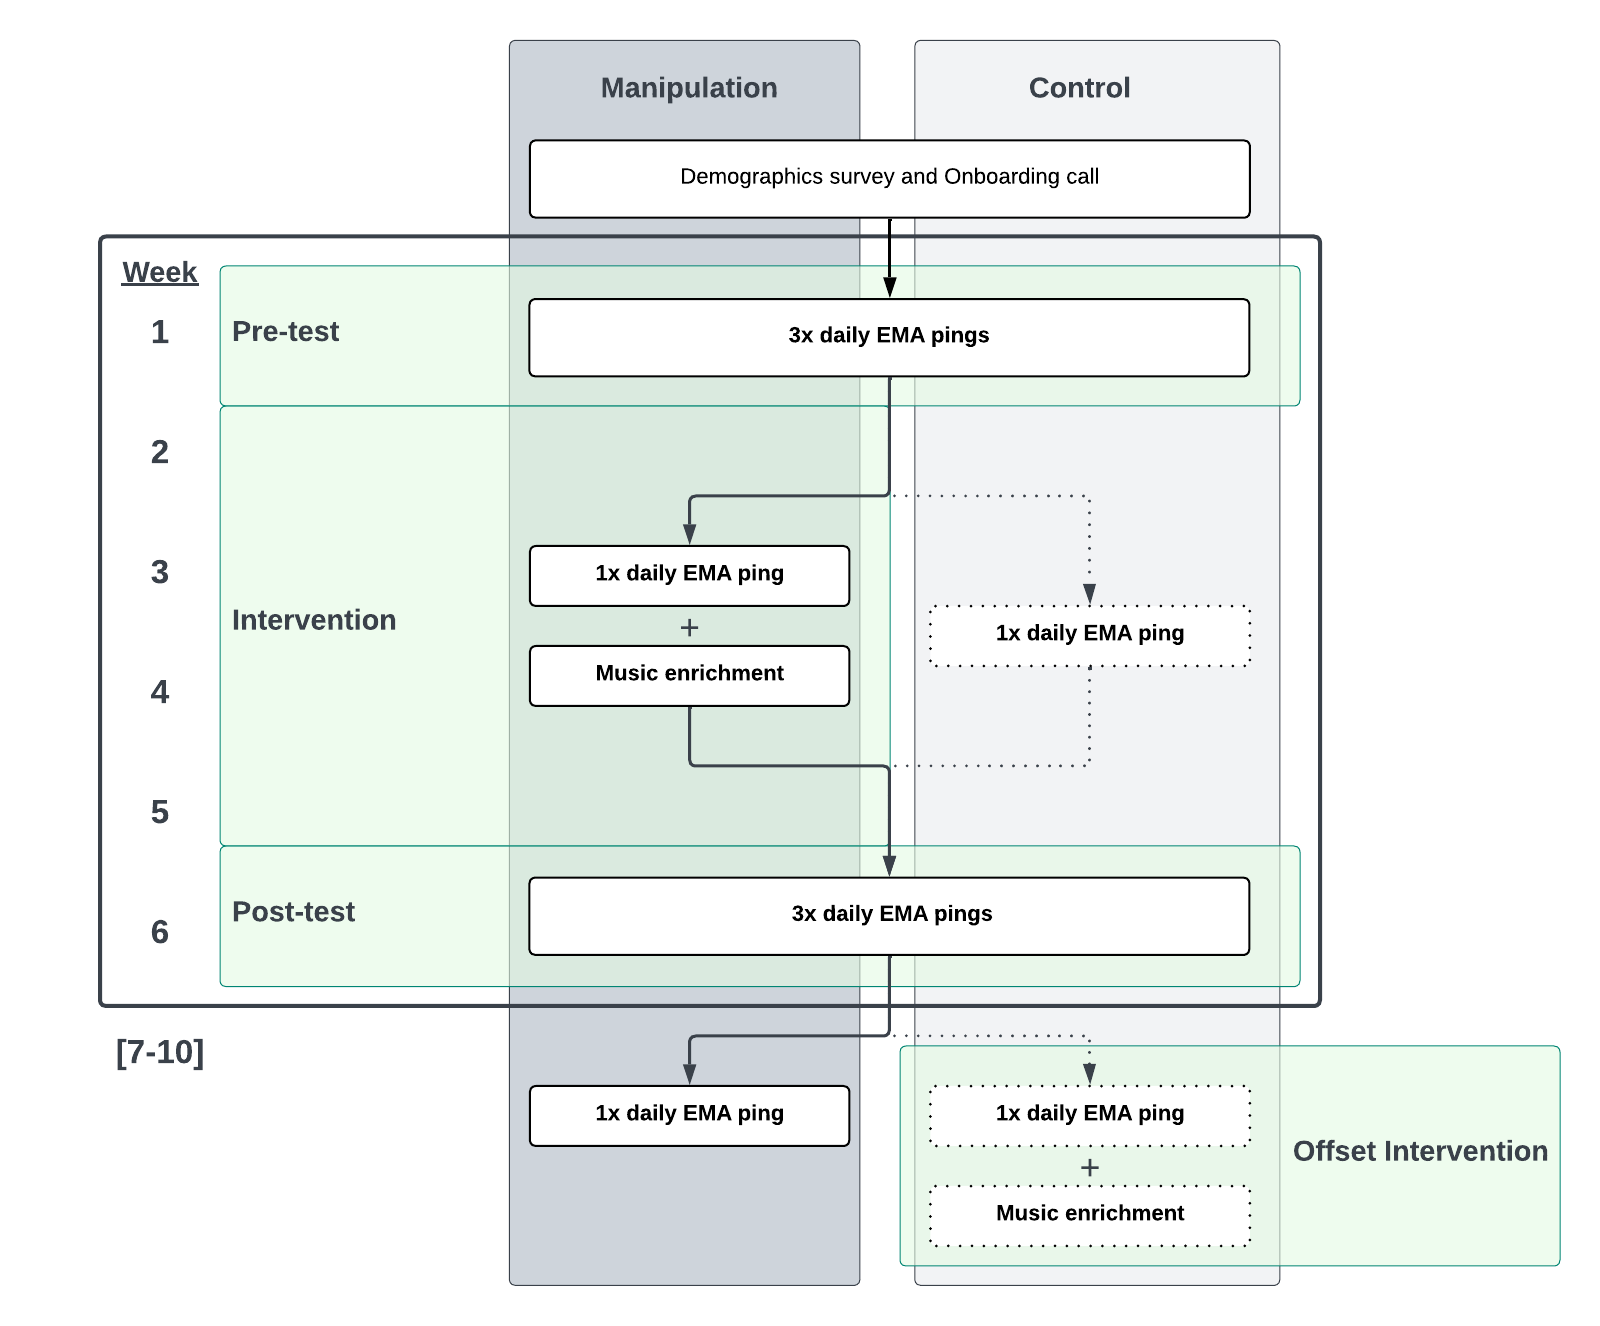
\includegraphics[width=0.9\linewidth,]{../viz/figure1} 

}

\caption{\textbf{Figure 1 | Structure of the experiment.} We conducted an offset-design randomized trial with a one-week pre-test, a four-week intervention, and a one-week post-test (see the areas highlighted in green). This main study period was followed by four further weeks of study participation, to accommodate the offset intervention period (for the control group). The left and right columns indicate the study flow for the manipulation and control groups, respectively. Both groups received the same number of EMA pings and followed identical procedures, except during the intervention period (weeks 2-5), during which the manipulation group participated in the music enrichment intervention along with their daily EMA pings, while the control group only completed the EMA pings and had no intervention.}\label{fig:figure 1}
\end{figure}

The study began with a one-on-one onboarding video call, where a
designated researcher provided an overview of the study, guided
participants in configuring their smartphones to receive EMA pings, and
answered any questions. Participants were required to be physically
present with their infants during the onboarding session to safeguard
against fraudulent participation, a common concern in online
developmental studies (\citeproc{ref-Perkel2020}{Perkel, 2020}). The
same researcher continued to serve as the participant's point of contact
throughout the rest of the study.

\subsection{Measures}\label{measures}

The primary measures of infant and caregiver health were collected via
EMA. We used a varied ping schedule, where caregivers received three EMA
surveys per day during the pre-test (week 1) and post-test (week 6),
delivered at randomly selected times in the morning, afternoon, and
evening; and one EMA survey per day at all other times during the study,
delivered at a randomly selected time during waking hours. In total,
caregivers received 98 EMA surveys across the 10 weeks of the study. We
did not require a minimum time between responses, so as to maximize the
amount of data we could analyze. EMA data collection was conducted
either via The Person Project, a smartphone app developed by authors
H.S. and D.T; or via Qualtrics surveys accessed via URLs in text
messages, distributed with Inclivio (\url{https://inclivio.com}).
Complete details about EMA methods are in Supplementary Text 2.

The EMA surveys measured characteristics of infant and caregiver health
in the 2-3 hours prior to the ping, including 12 items on (1)
\emph{infant mood}, measured by valence and arousal; (2) \emph{infant
distress and recovery}, assessed through a pictorial scale of infant
fussiness (\citeproc{ref-Adams2019}{Adams et al., 2019}), and details on
soothing techniques and duration for recovery; (3) \emph{caregiver mood
and stress}, measured by self-assessed valence, impact, and rationality
using the 3D Mind Model approach to mental state assessment
(\citeproc{ref-Thornton2020}{Thornton \& Tamir, 2020}), along with
self-reported levels of caregiving-related stress; and (4) \emph{musical
behavior}, measured by the frequency of caregivers' engagement with
focus behaviors (i.e., singing and music listening). Every ping included
an item asking whether the caregiver was with the infant during the 2-3
hours prior to the ping. If the caregiver answered ``No'', then no items
were presented concerning the infant's state (see Supplementary Text 3
for detail about this procedure and the full text of the EMA surveys).
We also included questions concerning the previous day, such as the
estimated frequency of infant-directed singing, the frequency of infant
night waking, and the duration taken to fall back asleep. During the
pre-test and post-test, these previous-day questions were only displayed
once per day. The full text of the EMA surveys is in Supplementary Text
3.

We also collected data in four longer-form surveys spread throughout the
study, for analysis in a different paper comparing EMA responses to
retrospective surveys; they are not reported here.

\subsection{Music Enrichment
Intervention}\label{music-enrichment-intervention}

The goal of the intervention was to increase the frequency of
infant-directed singing in daily life while also expanding caregivers'
repertoire of songs. We aimed to do so by teaching participants new
songs to sing at home and providing materials designed to encourage more
singing, in general, in the course of their caregiving. We did not
collect data regarding the exact content or acoustic features of songs
caregivers chose to sing to their infants, as we were interested in the
effects of increased singing in whatever form caregivers felt was
appropriate.

During the intervention, participants were given access to six
instructional videos of unfamiliar songs presented in karaoke style,
with lyrics synchronized to a bouncing ball indicating the rhythm (all
videos are available at
\url{https://github.com/themusiclab/musical-babies}). These were
displayed to participants either in The Person Project app or on YouTube
(i.e., at private URLs), depending on the type of EMA caregivers used
(see Supplementary Text 2). Three videos were sent at the start of the
intervention, with an additional three delivered halfway through. The
songs were sourced from vintage songbooks and online archives of folk
songs for children, then adapted for simplicity and ease of singing,
especially for caregivers with limited music training. This process
involved rewriting and arranging lyrics and melodies. The songs were
recorded and produced by members of the research team who had extensive
experience in early childhood music education (E.C., E.E., and S.A.M.).

Additionally, participants received an infant-friendly songbook of their
choice from a provided list (i.e., the Ditty Bird Musical Book series,
Cali's Books series), delivered to their homes at the outset of the
intervention. These books featured infant-pressable buttons that
activated song playback, accompanied by vibrant illustrations and
lyrics.

Last, to further motivate caregivers to sing more to their infants, we
sent weekly email newsletters to participants in the manipulation group
during the intervention. The newsletters introduced ideas to incorporate
singing into daily caregiving routines; highlighted the significance of
singing in infancy; and presented research findings relevant to the
benefits of musical parenting, in an easy-to-understand format. The
control group received the same newsletters in the offset intervention
period, but did not receive any newsletters during the main
intervention.

To sustain participants' engagement over the four-week intervention, the
research team maintained regular communication with participants via
text messages and emails. These check-ins provided study updates,
addressed any technical issues with the survey app, and reminded
participants to complete missed surveys. Caregivers were not discouraged
from singing outside of the intervention period; the intervention should
be understood as supplementing existing levels of singing in the home,
as opposed to suppressing such behaviors at non-intervention periods or
in the control group.

\subsection{Compliance}\label{compliance}

Participants responded to a median of 72 out of 98 scheduled pings, for
an overall response rate of 73.7\%, with a higher rate outside of the
pre- and post-test periods (i.e., when only receiving one EMA ping per
day; 78.4\%) than during the pre- and post-test periods (i.e., when
receiving three EMA pings per day; 67.9\%). This compliance rate is
comparable to those reported in other infant EMA studies, including
one-week studies with intensive daily pings
(\citeproc{ref-deBarbaro2023}{de Barbaro et al., 2023};
\citeproc{ref-Wenze2023}{Wenze et al., 2023};
\citeproc{ref-Franchak2019}{Franchak, 2019}) and longitudinal studies
lasting up to 16 weeks with less intensive pings
(\citeproc{ref-Allen2018}{Allen et al., 2018};
\citeproc{ref-Franchak2024}{Franchak et al., 2024};
\citeproc{ref-Corpuz2023}{Corpuz et al., 2023}). We then fit linear
models to test whether any demographic variables predicted compliance,
using a bootstrap procedure with 1000 resamples to obtain robust
estimates of the model coefficients.

Participants' response rates were unrelated to infant age at the start
of the study (\emph{p} = 0.44), total income (\emph{p} = 0.95), number
of siblings (\emph{p} = 0.56), or the caregivers' scores on a postpartum
depression inventory {[}Cox et al. (\citeproc{ref-Cox1987}{1987});
\emph{p} = 0.4{]}. The proportion of unanswered pings was slightly
higher in the control group, although this difference did not reach
significance at pre-test (\emph{p} = 0.29), intervention (\emph{p} =
0.09), or post-test (\emph{p} = 0.08). Given the comparable levels of
missingness in the two groups, we assume that nonresponse represents
missing data at random and did not attempt to account for missingness in
our analyses.

To assess responsiveness to EMA pings, we calculated response latency by
subtracting the time of the ping from the time participants opened the
survey on their smartphone. The median response latency was
approximately 20 minutes (high intensity weeks = 16 mins; low intensity
weeks = 23 mins); this analysis was only available for participants
whose pings were distributed by text message. A mixed-effects
time-series model that accounted for autoregression across the 6 weeks
of the study (with data averaged per day when multiple datapoints were
available) showed that latency increased with infant age (\(\beta\) =
0.09, \emph{SE} = 0.04, \emph{p} = 0.02).

\section{Results}\label{results}

\subsection{Music Enrichment Increases the Frequency of Infant-Directed
Singing}\label{music-enrichment-increases-the-frequency-of-infant-directed-singing}

We began by asking whether the intervention worked; namely, whether we
succeeded in increasing the frequency of infant-directed singing in the
manipulation group, relative to the control group. Two EMA items
addressed this question, in different ways.

First, every EMA ping included an item asking caregivers whether they
had sung to their infant in the preceding 2-3 hours. They could respond
``Yes'' or ``No''; the question was only asked of caregivers who
reported having been with their infant in the previous 2-3 hours (92.7\%
of all available data, see Measures). We dropped data where the
caregiver indicated in the same EMA ping that their infant was sick
(12.2\% of data). Here and throughout, we computed weekly average scores
using all available data from each participant.

Consistent with previous research using daylong audio recordings from
infants' home environments (\citeproc{ref-Hippe2024}{Hippe et al.,
2024}; \citeproc{ref-Lerma-Arregoces2024}{Lerma-Arregocés \&
Pérez-Moreno, 2024}; \citeproc{ref-Mendoza2021}{Mendoza \& Fausey,
2021}), music frequently featured in infants' and caregivers' lives even
prior to the intervention. At pre-test, caregivers reported having sung
to their infants in the previous 2-3 hours in 64.5\% of surveys
(\emph{SD} = 22.5\%). Caregivers also reported often playing recorded
music to their infants (\emph{M} = 38.4\%, \emph{SD} = 25.7\%) and
playing music for their own enjoyment (\emph{M} = 31.7\%, \emph{SD} =
27.3\%).

The intervention caused a clear increase in the frequency of
infant-directed song (Figure 2, left panel), with no difference between
groups at pre-test (proportion of ``Yes'' responses in manipulation
group: \emph{M} = 0.64, \emph{SD} = 0.24; in control group: \emph{M} =
0.65, \emph{SD} = 0.22; Wilcoxon Rank-Sum Test, \emph{W} = 1461,
\emph{p} = 0.85), and a large (\emph{d} = 0.61), statistically
significant difference at post-test (proportion of ``Yes'' responses in
manipulation group: \emph{M} = 0.77, \emph{SD} = 0.2; in control group:
\emph{M} = 0.64, \emph{SD} = 0.24; Wilcoxon Rank-Sum Test, \emph{W} =
1841, \emph{p} = 0.003). Note that during post-test, caregivers were no
longer actively being encouraged to sing more to their infants: week 5
was the last week of the intervention. The effect of the intervention
therefore persisted for at least one week beyond the intervention
itself.

A mixed-effects time-series model that accounted for autoregression
across the 6 weeks of the study (with data averaged per day when
multiple datapoints were available) showed a significant group-by-time
interaction (\(\beta\) = 0.26, \emph{SE} = 0.12, \emph{p} = 0.02). These
effects were specific to infant-directed singing, as we did not find
comparable interaction effects for other music-related variables that
were also reported in the same EMA surveys, such as playing recorded
music for the infant (\(\beta\) = -0.16, \emph{SE} = 0.12, \emph{p} =
0.18); or caregivers' personal music listening (\(\beta\) = 0.00,
\emph{SE} = 0.12, \emph{p} = 0.98) in the 2-3 hours preceding the EMA
ping.

\begin{figure}[p]
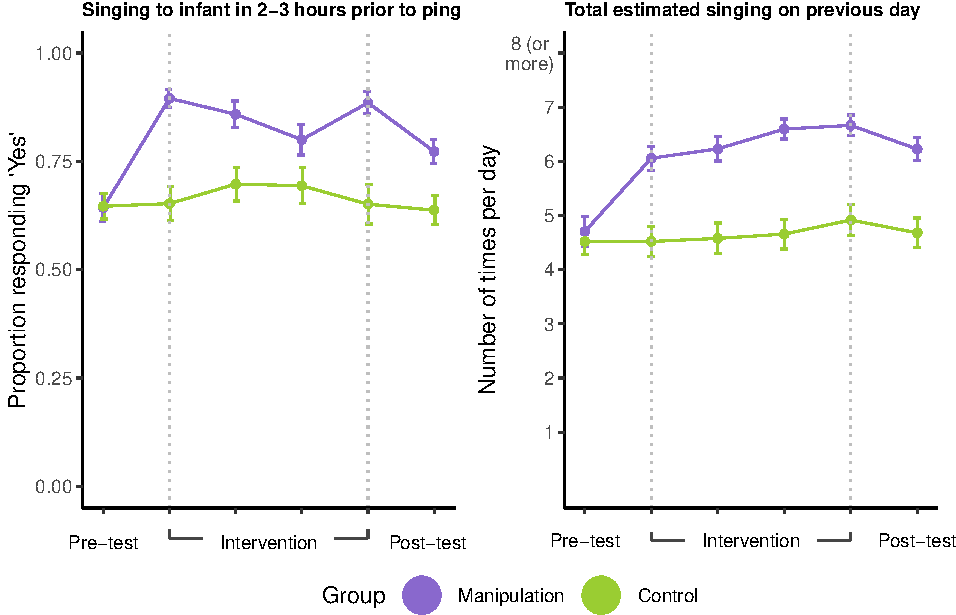
\includegraphics{MIPH_childdev_files/figure-latex/fig2-1} \caption{\textbf{Figure 2 | Music enrichment increases the frequency of infant-directed singing.} The plots depict responses to two items: ``Did you sing to [baby] in the last 2-3 hours?'', where ``[baby]'' was replaced by the infant's name (left panel), asked up to three times per day with response options ``Yes'' or ``No''; and ``If you had to guess, how many times did you sing to [baby] yesterday?'' (right panel), asked once per day with response options ranging from ``1'' to ``8 or more times''. There was a sharp increase in infant-directed singing for the manipulation group, but not the control group, as measured by both items; the increase persisted through the full intervention and was maintained in the post-test week. The tick marks on the $x$-axis indicate the study week; weeks 1 and 6 correspond to pre- and post-test, respectively, while weeks 2 through 5 span the intervention period. Note that for ease of visualization, here we plot weekly averages (points) and their corresponding standard errors of the mean (error bars), without accounting for temporal autocorrelation in responses over time. As such, the SEM values may be overestimating the precision of each estimate.}\label{fig:fig2}
\end{figure}

Notably, the absolute frequency of infant-directed singing was
substantial in the manipulation group: by the last week of the
intervention, the proportion of times a caregiver had recently sung to
their infant when they received an EMA ping was 0.89 -- almost all of
the time -- relative to 0.65 in the control group.

Second, caregivers reported an estimate of how many times they had sung
to their infant on the previous day (``If you had to guess, how many
times did you sing to {[}baby{]} yesterday?'') on an 8-point scale
ranging from ``1'' to ``8 or more times''. Here too we found a clear
effect of the intervention (Figure 2, right panel), with no group-level
difference at pre-test (Wilcoxon Rank-Sum Test, \emph{W} = 1582.5,
\emph{p} = 0.56), a significant difference at post-test (Wilcoxon
Rank-Sum Test, \emph{W} = 2118.5, \emph{p} \textless{} .001), and a
significant group-by-timepoint interaction (Mixed-effects time-series
model, \(\beta\) = 0.03, \emph{SE} = 0.01, \emph{p} \textless{} .0001)
indicating an estimated average increase of 0.28 singing episodes per
week in the manipulation group (roughly 3.5\% of the scale per week, for
a cumulative total of 20.8\% after the six weeks of intervention). While
caregiver reports summarizing the previous day's singing with an integer
may not be optimally precise, at the post-test period these effects
represented a 1.48 unit increase in absolute daily estimates of singing
behavior (\emph{SD} = 2.19).

Thus, convergent evidence demonstrates that the intervention succeeded
at its primary goal, namely, to experimentally manipulate caregivers'
infant-directed singing in daily life.

\begin{figure}[p]

{\centering 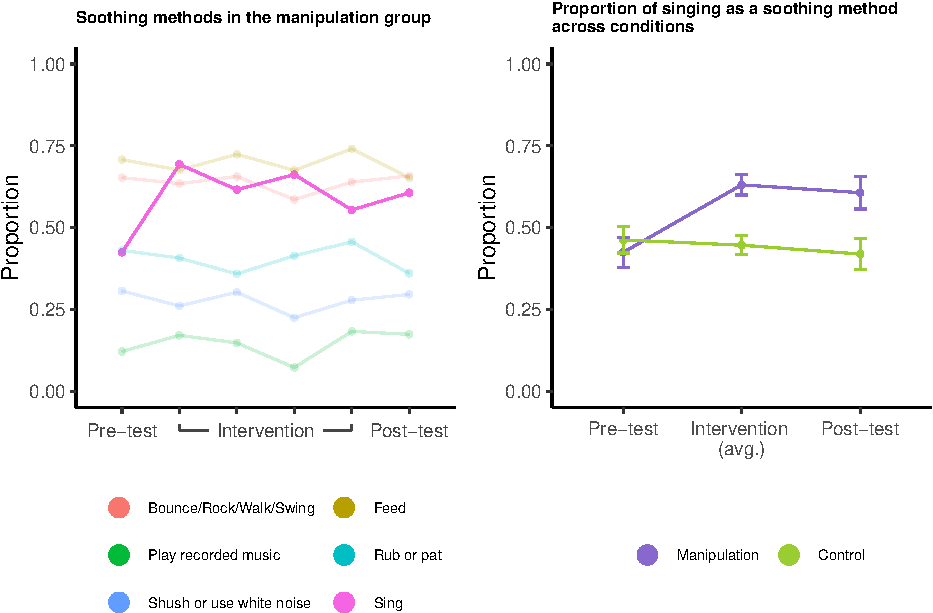
\includegraphics{MIPH_childdev_files/figure-latex/figure-3AB-1} 

}

\caption{\textbf{Figure 3 | Music Enrichment Alters Parent Responses to Infant Fussiness.} In each EMA ping, we asked the parent if their infant was fussy in the previous 2-3 hours; if they answered ``Yes'', then we asked how they attempted to soothe the infant. The left panel illustrates the proportion of responses in the manipulation group for six soothing techniques (of 12 available options; see Supplementary Text 3). Tick marks indicate the study week; weeks 1 and 6 correspond to pre- and post-test, respectively, whereas weeks 2 through 5 span the intervention period. Singing in response to fussiness was the only soothing technique out of 12 that showed a substantive increase in usage from pre- to post-test. This increase was specific to the manipulation group, as shown in the right panel, which rescales the data as a proportion of all responses and averages across the four intervention weeks (weeks 2-5). In the manipulation group, parents used singing in response to fussiness more than half of the time. The points indicate mean scores across the given week(s) and error bars denote standard errors of the mean.}\label{fig:figure-3AB}
\end{figure}

\subsection{Music Enrichment Increases the Use of Singing Specifically
in the Context of Soothing
Infants}\label{music-enrichment-increases-the-use-of-singing-specifically-in-the-context-of-soothing-infants}

Given the well-known role of music in soothing or calming infants (e.g.,
\citeproc{ref-Bainbridge2021}{Bainbridge et al., 2021}), we wondered
whether the intervention had not only general effects on the use of
infant-directed singing, but also specific effects in the context of
soothing.

It did. In each EMA survey, we asked participants if their infant was
fussy in the last 2-3 hours. If so, they indicated all soothing
techniques they used in response, from a list of 12 different techniques
(e.g., feeding, changing a diaper, shushing, playing recorded music,
singing; the full list is in Supplementary Text 3). Parents reported
that their infant was fussy (and not sick) in 41\% of instances.

While the use of most soothing techniques remained more-or-less constant
over the course of the study, in the manipulation group there was a
large increase in the proportion of time caregivers used singing in
response to fussy infants (Figure 3, left panel; pre-test: \emph{M} =
0.42, \emph{SD} = 0.33; average across intervention: \emph{M} = 0.63,
\emph{SD} = 0.40; post-test: \emph{M} = 0.61, \emph{SD} = 0.35). While
singing was the third most frequently used soothing technique among the
12 different techniques (both at pre-test and overall), following
movement-based soothing (i.e., picking-up, bouncing, rocking, or
swinging) and feeding, singing was the only technique with increased
caregiver use as a result of the intervention, an increase of 19
percentage points from pre-test to post-test (Wilcoxon Signed Rank Test,
\emph{V} = 769, \emph{p} = 0.001).

No such increase was observed in the control group, however; there, the
singing response stayed relatively flat (Wilcoxon Signed Rank Test,
\emph{V} = 365.5, \emph{p} = 0.4; Figure 3, right panel). The
cross-group difference at post-test was statistically significant
(Wilcoxon Rank-Sum Test, \emph{W} = 1642.5, \emph{p} = 0.006). Notably,
we did not observe a group-level difference at post-test in the
frequency of playing recorded music to infants, indicating that the
effect did not reflect a general increase in the use of music to soothe
infants (Wilcoxon Rank-Sum Test, \emph{W} = 1274.5, \emph{p} = 0.85).
Rather, it was specific to singing.

Thus, music enrichment not only increased the overall use of
infant-directed singing in daily life, but specifically influenced how
caregivers responded to infant fussiness. We note here that caregivers
were not explicitly instructed to use music in the context of soothing.
The newsletters provided general suggestions for incorporating music
into many different infant care contexts, one of which was soothing; the
specific increase of the use of music in this context suggests that the
decision to use music for soothing was likely an intuitive one.

\subsection{Infant-Directed Singing Improves Infant Mood but not
Caregiver
Mood}\label{infant-directed-singing-improves-infant-mood-but-not-caregiver-mood}

As music has been shown to affect a variety of affect- and
arousal-related variables in infants in the short-term (e.g.,
\citeproc{ref-Bainbridge2021}{Bainbridge et al., 2021};
\citeproc{ref-Cirelli2020}{Cirelli \& Trehub, 2020};
\citeproc{ref-Corbeil2016}{Corbeil et al., 2016}), a key question for
this randomized trial is whether such effects are cumulative. Does music
enrichment produce lasting effects on infant affect?

To study this question, we focused primarily on caregiver evaluations of
infant mood, reported using a sliding scale from Negative (0) to
Positive (100). In each EMA survey, caregivers rated their infant's mood
during the last 2-3 hours. Caregivers only responded if they had been
with their infant during that time.

Importantly, this item does \emph{not} measure caregivers' perceptions
of infants' mood in response to singing. Rather, the item measures
perceptions of infant mood \emph{in general}.

To account for participant variability in scale usage, we
\emph{z}-scored mood ratings within participants. We then computed a
weekly average score for each infant. Consistent with other research
showing less frequent crying as infants grow older
(\citeproc{ref-Barr1990}{Barr, 1990}), infants showed improvements in
mood from pre- to post-test, on average (mean difference = 0.25;
Wilcoxon Signed Rank Test, \emph{V} = 4128, \emph{p} \textless{} .0001).

These improvements were moderated by manipulation group, however (Figure
4, left panel). At pre-test the two groups did not differ (in
\emph{z}-scores, manipulation group: \emph{M} = -0.10, \emph{SD} = 0.41;
control group: \emph{M} = -0.11, \emph{SD} = 0.30; Wilcoxon Rank-Sum
Test, \emph{W} = 1520, \emph{p} = 0.58), but at post-test, the
intervention had caused a significant difference in infant mood, with
the manipulation group approximately 0.18 standard deviations higher
(manipulation group: \emph{M} = 0.24, \emph{SD} = 0.32; control group:
\emph{M} = 0.06, \emph{SD} = 0.32; Wilcoxon Rank-Sum Test, \emph{W} =
1822, \emph{p} = 0.004).

A mixed-effects time-series model (using untransformed data and daily
averages of individuals' responses when multiple datapoints were
available) that accounted for autoregression showed a significant
group-by-time interaction (\(\beta\) = 0.18, \emph{SE} = 0.05, \emph{p}
\textless{} .001). In the manipulation group, each week of intervention
was associated with a 1.56-unit increase in the 100-point mood scale for
infants in the manipulation group (\emph{p} \textless{} .001), or
roughly one tenth of a \emph{SD} increase per week of intervention.

We tested the robustness of this effect by asking whether it repeated in
two subsets of the main sample: a first cohort, recruited mainly in the
United States from February to June 2023; and a second cohort, recruited
mainly in New Zealand from June to December 2023. Mixed-effects
time-series models revealed the same expected group-by-time interaction
in both the first (\(\beta\) = 0.12, \emph{SE} = 0.06, \emph{p} = 0.04)
and second cohorts (\(\beta\) = 0.32, \emph{SE} = 0.10, \emph{p} =
0.001).

\begin{figure}[p]
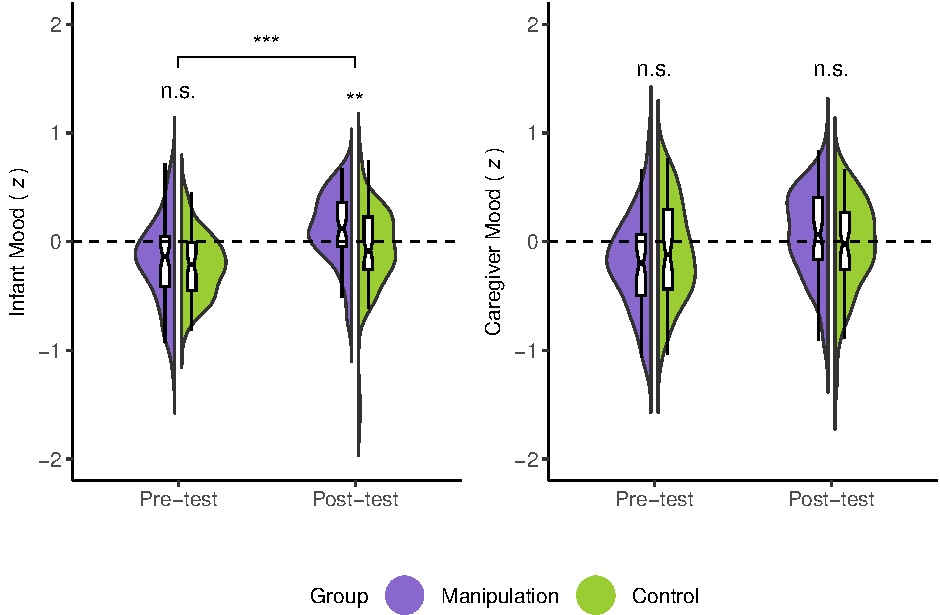
\includegraphics{MIPH_childdev_files/figure-latex/fig4-1} \caption{\textbf{Figure 4 | Music enrichment improves infant mood but not caregiver mood.} In each EMA ping, caregivers were asked to report their infant's mood and their own mood during the previous 2-3 hours, both on a 100-point slider anchored at ``Very negative'' and ``Very positive''. We normalized responses within participants to account for individual differences in scale use. While average mood of infants in the two groups did not differ at pre-test, it did at post-test, with significantly more positive mood reports in the manipulation group (left panel). We did not observe the same pattern for caregiver mood (right panel). The half-violins depict the distributions of weekly mean mood ratings from each of the two groups, weighted by participant. The shaded area in the half-violins represent kernel density estimates; the boxplots denote the median (horizontal line), 95\% confidence interval (notches), and interquartile range (edges of the boxes). The significance stars above the violins denote the between-groups comparison at a given time point. The horizontal bar denotes the significant group-by-time interaction in the time-series model. $^{\ast}p < 0.05$, $^{\ast\ast}p < 0.01$, $^{\ast\ast\ast}p < 0.001$.}\label{fig:fig4}
\end{figure}

Caregivers also rated how energetic their infants were in the previous
2-3 hours, using a similar scale to the mood item; we found no
corresponding effects on this measure, suggesting the effects of music
enrichment are specific to infant mood and do not generalize to infant
arousal.

We proceeded by analyzing data concerning caregiver mood, for two
reasons. First, improvements to infant mood might well translate to
improvements in caregiver mood, since happier infants are easier to look
after than fussier ones. Second, a concern with the infant mood result
is the potential for contamination in caregiver self-reports: they might
erroneously report happier infants when they themselves felt happier.
Because this experiment relies on caregiver EMA data, we are unable to
directly assess infant mood in isolation from the caregiver.

We addressed these issues with several analyses of caregivers' responses
to ratings of their own mood, completed in the same EMA surveys and
using the same normalization approach as the infant mood item. In
contrast to infant mood, we found no differences between groups at
pre-test (Figure 4, right panel; manipulation group: \emph{M} = -0.15,
\emph{SD} = 0.46; control group: \emph{M} = -0.02, \emph{SD} = 0.48;
Wilcoxon Rank-Sum Test, \emph{W} = 1213, \emph{p} = 0.18) or post-test
(manipulation group: \emph{M} = 0.14, \emph{SD} = 0.43; control group:
\emph{M} = 0.03, \emph{SD} = 0.48; Wilcoxon Rank-Sum Test, \emph{W} =
1543, \emph{p} = 0.29). This absence of effect suggests that the effect
of music enrichment on caregiver self-reports of infant mood does not
erroneously represent an effect on caregiver mood.

Infant mood and caregiver mood were moderately and positively
correlated, however (Spearman's rank correlation; \emph{r} = 0.39,
\emph{p} \textless{} .0001), and adding caregiver mood as a predictor to
the mixed model regressing condition and day number on infant mood
weakened the time-by-group interaction enough that it no longer reached
statistical significance (\emph{p} = 0.09). While the correlation
between infant and caregiver mood could indicate a true relation between
these variables, a response bias, or both, we found no evidence for a
difference in the size of the correlation across the manipulation and
control groups (\(\beta\) = 0.01, \emph{p} = 0.59); this suggests that
any reporting biases, should they exist, are not attributable to the
intervention.

To further assess the degree of potential confounding between infant and
caregiver mood reports, we tested whether each of the infant and
caregiver mood self-reports correlated with other measures that should
be expected to be more strongly linked to caregiver mood than infant
mood. Two variables in the daily EMA surveys met this criterion: a
measure of how socially connected caregivers felt (from ``Very lonely''
to ``Very connected'') and a measure of the perceived stress of
caregiving (``How stressful have you found parenting in the last 2-3
hours?'').

The association of social connection and caregiver mood (\(\beta\) =
0.44, \emph{p} \textless{} .0001) was both stronger and in the opposite
direction of the association between social connection and infant mood
(\(\beta\) = -0.08, \emph{p} = 0.02; interaction: \(\beta\) = 0.002,
\emph{p} \textless{} .0001; autoregressive time series model with
untransformed mood data). Similarly, while both infant (\(\beta\) =
-0.017, \emph{p} \textless{} .0001) and caregiver mood (\(\beta\) =
-0.019, \emph{p} \textless{} .0001) predicted how stressful caregivers
found parenting, the interaction between the two mood variables was
statistically significant (\(\beta\) = 0.0001, \emph{p} \textless{}
.0001), indicating a significantly stronger relation between caregiver
mood and parenting stress than between caregiver mood and infant mood.
These results suggest that our measures of infant mood and caregiver
mood tapped into substantively different phenomena, and were not fully
confounded.

In sum, we found a causal effect of music enrichment on infant mood, but
not caregiver mood, despite the two mood measures being correlated with
one another. It is possible that increasing the frequency of
infant-directed singing may improve \emph{both} infants' and caregivers'
moods, whether directly (e.g., singing makes caregivers feel positive)
or indirectly (e.g., having a happier infant makes caregivers feel
positive). If so, putative effects on caregiver mood are small enough
that they could not be reliably detected in this brief intervention
study.

\section{Discussion}\label{discussion}

We report evidence that a brief singing intervention increases the
frequency of infant-directed singing, that caregivers intuitively extend
this musical behavior specifically to the context of soothing their
infants, and that these changes in the home musical environment cause
improvements to infant mood in general. This suggests that the immediate
effects of music on infants' moods (e.g.,
\citeproc{ref-Bainbridge2021}{Bainbridge et al., 2021};
\citeproc{ref-Cirelli2020}{Cirelli \& Trehub, 2020};
\citeproc{ref-Cirelli2020a}{Cirelli et al., 2020};
\citeproc{ref-Corbeil2016}{Corbeil et al., 2016};
\citeproc{ref-Shenfield2003}{Shenfield et al., 2003}) may be cumulative,
leading to longer-term effects.

Importantly, the effect of the music enrichment intervention on infant
mood was detected in EMA data collected \emph{regardless of whether the
caregiver had recently sung to the infant} (i.e., as opposed to
measuring infants' mood responses to singing in particular). This
implies that infant-directed singing improved infant mood \emph{in
general}, in a one-week post-test period that followed the intervention
(at which time we were no longer telling caregivers to sing to their
infants). The present findings therefore substantiate a causal relation
between an enriched musical environment and general improvements in
infant mood.

Moreover, while this result is supported only by caregiver-observational
data, several considerations suggest that the findings reflect robust
changes in infant affect. First, the data were collected with EMA,
instead of retrospective surveys, and therefore are unlikely to be
contaminated by recall bias (\citeproc{ref-Stone2002}{Stone \& Shiffman,
2002}; \citeproc{ref-Reis2012}{Reis, 2012}). Second, the results largely
replicated internally, in two separate samples recruited in two
different countries, and therefore are unlikely to reflect the
caregiving practices of only one community. Third, we found no
corresponding effect of the intervention on caregiver mood, suggesting
that caregivers' self-reports of infant mood did not simply reflect
caregivers' own mood, as they might in the presence of a reporting bias.
Fourth, the modest correlation between caregiver reports of infant mood
and their own mood was of a comparable size in both the manipulation and
control groups, suggesting that a social-desirability effect (e.g.,
where parents who had experienced the intervention reported higher
infant mood because they felt obligated to do so) did not account for
the main effects. Future studies can more precisely investigate the
validity of infant mood assessment via EMA by supplementing the method
with direct, independent lab-based or home-based observations of infant
mood and behavior, psychophysiological measures of infant arousal, and
so on.

Infant mood is an important issue for caregivers as it is closely linked
to parenting stress (\citeproc{ref-Oddi2013}{Oddi et al., 2013}),
caregiver-infant bonding and attachment (\citeproc{ref-Nolvi2016}{Nolvi
et al., 2016}; \citeproc{ref-Takacs2020}{Takács et al., 2020}), and
subsequently the infants' social and emotional development
(\citeproc{ref-Steele2008}{Steele et al., 2008};
\citeproc{ref-Shaw2005}{Shaw \& Dallos, 2005}). These associations raise
the possibility that general improvements in infant mood, caused by
altering the home music environment in young families, could
subsequently cause other positive health-related outcomes. While we did
not observe any such effects here (such as an improvement in caregiver
mood), we note that this study had only a brief (4-week), low-intensity,
self-directed intervention. A longer-term, higher-intensity
intervention, perhaps with direct music instruction from a qualified
teacher, may well uncover more widespread effects. These could
potentially generalize to other health domains that are tightly related
to caregivers' well-being, such as the frequency of infant night waking,
the duration of crying bouts, the ease with which caregivers can calm
their infants when upset, or levels of caregiver stress.

Infant-directed singing is a multifaceted mode of communication and
interaction, including a variety of distinct musical attributes, such as
exaggerated melodic contours, high pitch variability, repetitive
rhythmic patterns (e.g., \citeproc{ref-Malloch2009}{Malloch \&
Trevarthen, 2009}; \citeproc{ref-Hilton2022a}{Hilton et al., 2022}); in
conjunction with other caregiving behaviors, such as increased physical
proximity, infant-directed attention, touch, rocking, infant-directed
speech (\citeproc{ref-Mehr2017a}{Mehr \& Krasnow, 2017};
\citeproc{ref-Mehr2021}{Mehr et al., 2021};
\citeproc{ref-Trehub2019}{Trehub \& Gudmundsdottir, 2019}). We cannot
yet know which of these specific characteristics or behaviors are the
ones that caused improvements in infant mood, as the intervention likely
altered all of them. Future randomized trials that include active
control groups may determine the degree to which \emph{singing}
specifically alters infant temperament, over and above the many positive
caregiving behaviors that are associated with singing.

We note that prior to the intervention, music was already well
integrated into daily routines in many families in our sample, with
parents reporting several instances of singing to their infants each
day, on average. This aligns with previous research highlighting the
widespread use of music, especially singing, in infancy
(\citeproc{ref-Yan2021}{Yan et al., 2021};
\citeproc{ref-Custodero2003a}{Custodero et al., 2003};
\citeproc{ref-Fancourt2018}{Fancourt \& Perkins, 2018c};
\citeproc{ref-Ilari2005}{Ilari, 2005}), although a recent report using
more precise measurement of the home auditory environment (via daylong
audio recordings) found surprisingly low rates of music exposure across
infancy (\citeproc{ref-Hippe2024}{Hippe et al., 2024}). Despite the
pre-existing musical engagement, the brief intervention led to a further
increase in both the frequency of daily singing and its use for soothing
fussy infants, as reflected in EMA reports, while no significant changes
in music listening frequency were observed. If the limited musical input
reported by Hippe and colleagues (\citeproc{ref-Hippe2024}{2024}) better
reflects infants' environmental norms, the potential effects of music
enrichment interventions may be underestimated here, in fact.

We also note several limitations of our sample. Demographic factors,
such as education and socioeconomic status, can closely shape parenting
behaviors and attitudes (\citeproc{ref-Bradley2002}{Bradley \& Corwyn,
2002}), including their everyday use of music with infants. As the
majority of our participants were White, highly educated and socially or
economically advantaged, it is not yet clear whether the longer-term
effects of music enrichment will generalize to other populations. The
inclusion of more diverse samples is essential for future studies.

On a methodological note, our findings demonstrate the feasibility of
long-term EMA studies in young infants and their caregivers. We observed
that consistent engagement in the study over a 10-week period, while
learning from the intervention and integrating that learning into
caregivers' daily routines with young infants, was manageable for
caregivers, based on the low level of attrition and high level of
compliance. EMA is commonly used in studies of adults but is relatively
underused by developmentalists; when used, studies are typically short,
spanning less than 2 weeks (e.g., \citeproc{ref-deBarbaro2023}{de
Barbaro et al., 2023}; \citeproc{ref-Franchak2019}{Franchak, 2019};
\citeproc{ref-Wenze2023}{Wenze et al., 2023}). While latency to ping
response did vary in our data, including an increase in response time as
infants grew older, very few families dropped out of the study (i.e., a
retention rate of 92\%), despite our asking caregivers to respond to
nearly 100 surveys in 10 weeks.

We believe the EMA method complements traditional laboratory-based or
retrospective survey designs because it enables the collection of
repeated, naturalistic observations of infant and caregiver behaviors
and psychological states, which fluctuate both daily and over extended
periods. Although infant EMA research is limited by infants' inability
to report on their own behaviors and mental states (i.e., caregivers are
responsible for assessing and reporting their infants' moods), analyses
of the relations between caregiver-reported infant mood and caregiver
mood may provide some optimism that the recruitment of caregivers as
``scientist-observers'' does not imply compromised data quality. As
such, we encourage the research community to consider EMA in infant
studies.

Last, we note that the primary caregivers of young infants studied here
were quite happy to engage with a multi-week music intervention, despite
having relatively little music training, on average; and despite being
presumably quite busy, stressed-out primary caregivers of young infants.
At the end of the study, the vast majority of caregivers reported that
they would continue singing to their infants after the study (90.3\%),
and self-reported their overall experience in the study as positive,
particularly appreciating the opportunities to actively incorporate
music into their daily lives and experience the positive impacts singing
had on their infants as well as themselves (see Supplementary Text 4 for
further information and results from the exit survey). These findings,
combined with the ease of carrying out the intervention, its very low
cost, and its other reported effects, suggest a strong potential for
music enrichment to improve infant and caregiver health.

\clearpage

\section*{End notes}\label{end-notes}
\addcontentsline{toc}{section}{End notes}

\subsection*{Data, Code, and Materials
Availability}\label{data-code-and-materials-availability}
\addcontentsline{toc}{subsection}{Data, Code, and Materials
Availability}

A fully reproducible manuscript; data; analysis and visualization code;
and other materials are available at
\url{https://github.com/themusiclab/musical-babies}. This repository
will be permanently archived on Zenodo at the time of publication.
Analyses were exploratory and not preregistered.

\subsection*{Acknowledgments}\label{acknowledgments}
\addcontentsline{toc}{subsection}{Acknowledgments}

We thank the families for their participation; Stacey Sinclair, Epi
Torres, Katie Ippolito, and Nicole Shelton for their support on The
Person Project; Anna Bergson, S. Atwood, and Anya Keomurjian for
research assistance; Danilo Lombardo for assisting with producing music
enrichment intervention materials; and the members of The Music Lab for
helpful discussions and feedback. Jerome Kagan, who passed away in May
2021, contributed early ideas that led to this work, in lively
conversation with S.A.M.

\subsection*{Funding}\label{funding}
\addcontentsline{toc}{subsection}{Funding}

This research was supported by grants from the US National Institutes of
Health (DP5OD024566 and R21HD113998), the Royal Society of New Zealand
Te Apārangi (Rutherford Discovery Fellowship RDF-UOA2103), and the
University of Auckland (Research Development Fund and Early Career
Research Excellence Award) to S.A.M. The Person Project was supported by
a grant from Princeton University (Eric and Wendy Schmidt Transformative
Technology Fund) to D.I.T.

\subsection*{Author Contributions}\label{author-contributions}
\addcontentsline{toc}{subsection}{Author Contributions}

\begin{itemize}
\tightlist
\item
  S.A.M. conceived of the research, provided funding, supervised the
  study team, and coordinated all project activities.
\item
  D.I.T. provided funding for the Person Project data collection
  platform.
\item
  E.C., L.Y., E.E., B.M., and S.A.M. contributed to study design and
  materials development, including the music enrichment intervention.
\item
  E.L., M.B., P.B., and B.M. provided research assistance.
\item
  C.B.H. led implementation of the study on the Person Project data
  collection platform, with additional contributions from H.S., S.A.M.,
  and D.I.T.
\item
  E.L. and S.A.M. implemented the study on the Inclivio data collection
  platform.
\item
  E.C., L.Y., E.E., and E.L. collected data and managed all
  communication with participants.
\item
  L.Y. wrote analysis code, with additional contributions from E.C.,
  C.B.H., and S.A.M.
\item
  C.B.H. conducted a review of the code and statistical analyses.
\item
  L.Y., E.C., and S.A.M. designed the figures.
\item
  E.C., L.Y., and S.A.M. wrote the manuscript and all authors edited or
  approved it.
\end{itemize}

\newpage

\section*{Online Supplementary
Information}\label{online-supplementary-information}
\addcontentsline{toc}{section}{Online Supplementary Information}

\subsection*{Supplementary Text 1: Excluded
Participants}\label{supplementary-text-1-excluded-participants}
\addcontentsline{toc}{subsection}{Supplementary Text 1: Excluded
Participants}

Demographic information for the excluded participants is reported in
Supplementary Table 2, so as to enable a comparison to the demographics
of the included participants. The small number of excluded participants
precludes the use of inferential statistics comparing these groups, as
any such comparison would have low statistical power.

Note, however, that there appeared to be a difference in caregivers'
mental health across included vs.~excluded participants. At the start of
the study, the caregivers who had given birth to the infant (95\% of
participants) completed the Edinburgh Postnatal Depression Scale
(\citeproc{ref-Cox1987}{Cox et al., 1987}), a screening tool for
postpartum depression; 17\% of included participants scored above the
screening cut off (10 out of 30), compared to 33\% of excluded
participants. Caregivers experiencing negative mental health outcomes
may be less likely to continue participation in a longitudinal study.

\subsection*{Supplementary Text 2: EMA
Distribution}\label{supplementary-text-2-ema-distribution}
\addcontentsline{toc}{subsection}{Supplementary Text 2: EMA
Distribution}

We used two different methods for EMA distribution, which had minor
differences in user experience: one was a standalone smartphone app that
participants downloaded on their phones, while the other distributed EMA
surveys by text message. Despite these differences, both methods
delivered the same survey content. The choice of method is unlikely to
have influenced scientific outcomes of this work, as comparable numbers
of participants in the manipulation (\(n_{app}\) = 29, \(n_{text}\) =
25) and control groups (\(n_{app}\) = 44, \(n_{text}\) = 12) used each
EMA method. The method assignment was determined chronologically, with
the first cohort (recruited mainly in the United States) using the
Person Project, and the second cohort (recruited mainly in New Zealand)
using Inclivio.

During the pre-test and post-test, caregivers received three pings a
day, spaced at least 2 hours apart, in the morning (9:00am-11:30am),
afternoon (1:30pm-4:00pm) and evening (6:00pm-8:30pm). During these
periods, items that were only asked once per day (see Supplementary Text
3) were displayed in pings arriving before 11:30am for participants
using The Person Project and in the first ping of the day for
participants using Inclivio. For the Person Project participants,
once-a-day questions about the previous day were only displayed if the
ping arrived before 11:30am, meaning that on low frequency days, a ping
arriving after 11:30am would not ask about the previous day. This was
modified for Inclivio participants: the first Inclivio notification of
the day included questions about the previous day, regardless of
delivery time.

At all other times, participants received one daily EMA survey ping
between 8:30am-8:30pm on the Person Project, and between 9:00am-8:30pm
on Inclivio. Each survey took approximately two minutes to complete.
Participants were encouraged to complete the survey promptly upon the
arrival of the ping.

Details of the two distribution methods follow.

\subsubsection*{The Person Project}\label{the-person-project}
\addcontentsline{toc}{subsubsection}{The Person Project}

In this EMA distribution method, participants completed surveys in a
smartphone app built on the React programming library for iOS and
Android. This app presented survey items in JavaScript; participants
were prompted to complete them via push notifications; and securely
stored their responses in a PostgreSQL database, implemented via Ruby on
Rails on Amazon Web Services. Upon an arrival of a ping, participants
accessed the surveys by tapping the notification. If participants could
not complete the survey immediately, they could still access it through
their notification history on the smartphone. EMA pings did not expire.

\subsubsection*{Inclivio}\label{inclivio}
\addcontentsline{toc}{subsubsection}{Inclivio}

In this EMA distribution method, participants received text messages
that each contained a URL leading to a Qualtrics survey. Inclivio
facilitated participant enrollment, distributed the text messages, and
transmitted participant identifiers and other relevant data (e.g., time
indicators, custom values to pipe into our survey questions) to
Qualtrics, as in previous EMA studies using the platform
(\citeproc{ref-Kuczynski2024}{Kuczynski et al., 2024};
\citeproc{ref-Dora2024}{Dora et al., 2024}). EMA pings expired after 4
hours.

\subsection*{Supplementary Text 3: EMA Survey
Content}\label{supplementary-text-3-ema-survey-content}
\addcontentsline{toc}{subsection}{Supplementary Text 3: EMA Survey
Content}

This section reproduces the text of all items in the EMA surveys; the
same content was presented across the two EMA distribution methods, with
minor differences in the appearance of each item. The text ``BABY'' was
replaced with the infant's first name.

\textbf{1. Please report how YOU have been feeling in the last 2-3 hours
on the following scales.}

\begin{enumerate}
\def\labelenumi{\alph{enumi}.}
\tightlist
\item
  How positive have you been feeling? {[}slider{]} Very negative ---
  Very positive
\item
  How energetic have you been feeling? {[}slider{]} Very lethargic ---
  Very energetic
\item
  How socially connected have you been feeling? {[}slider{]} Very lonely
  --- Very connected
\item
  Have you been spending more time thinking or feeling? {[}slider{]}
  Thinking --- Feeling
\end{enumerate}

\textbf{2. How stressful have you found parenting in the last 2-3
hours?}

\begin{enumerate}
\def\labelenumi{\alph{enumi}.}
\tightlist
\item
  Not stressful at all
\item
  A bit stressful
\item
  Somewhat stressful
\item
  Very stressful
\end{enumerate}

\textbf{3. Last night, how many times did BABY wake up after s/he fell
asleep?} {[}\emph{This item was only included in the first ping of the
day.}{]}

\begin{enumerate}
\def\labelenumi{\alph{enumi}.}
\tightlist
\item
  Slept through the whole night
\item
  Woke up once
\item
  Woke up twice
\item
  Woke up three or more times
\end{enumerate}

{[}\emph{If baby woke up}{]} \textbf{3.1 When BABY woke up during the
night, how long did it take for him/her to fall back asleep?}

\begin{enumerate}
\def\labelenumi{\alph{enumi}.}
\tightlist
\item
  Less than 2 minutes
\item
  3-8 minutes
\item
  9-15 minutes
\item
  More than 15 minutes
\end{enumerate}

\textbf{4. If you had to guess, how many times did you sing to BABY
yesterday?} {[}\emph{This item was only included in the first ping of
the day.}{]}

{[}slider{]} 1 --- 8 or more times

\textbf{5. Were you with BABY in the last 2-3 hours?}

\begin{enumerate}
\def\labelenumi{\alph{enumi}.}
\tightlist
\item
  Yes
\item
  No
\end{enumerate}

{[}\textbf{\emph{If parents answered ``No'' to this question, the survey
ended}}{]}

\textbf{6. Do you think BABY is feeling sick today?}

\begin{enumerate}
\def\labelenumi{\arabic{enumi}.}
\tightlist
\item
  Yes
\item
  No
\end{enumerate}

\textbf{7. How would you describe BABY's mood in the last 2-3 hours?}

\begin{enumerate}
\def\labelenumi{\alph{enumi}.}
\tightlist
\item
  Very negative --- Very positive {[}continuous scale{]}
\item
  Very passive/calm --- Very aroused/active {[}continuous scale{]}
\end{enumerate}

\textbf{8. In the last 2-3 hours, was BABY at all distressed or fussy?}

\begin{enumerate}
\def\labelenumi{\alph{enumi}.}
\tightlist
\item
  Yes
\item
  No
\end{enumerate}

\textbf{9.1.} {[}\emph{If baby was fussy}{]} \textbf{How distressed or
fussy was BABY?} (Scale adapted from Adams et al.~(2019).)

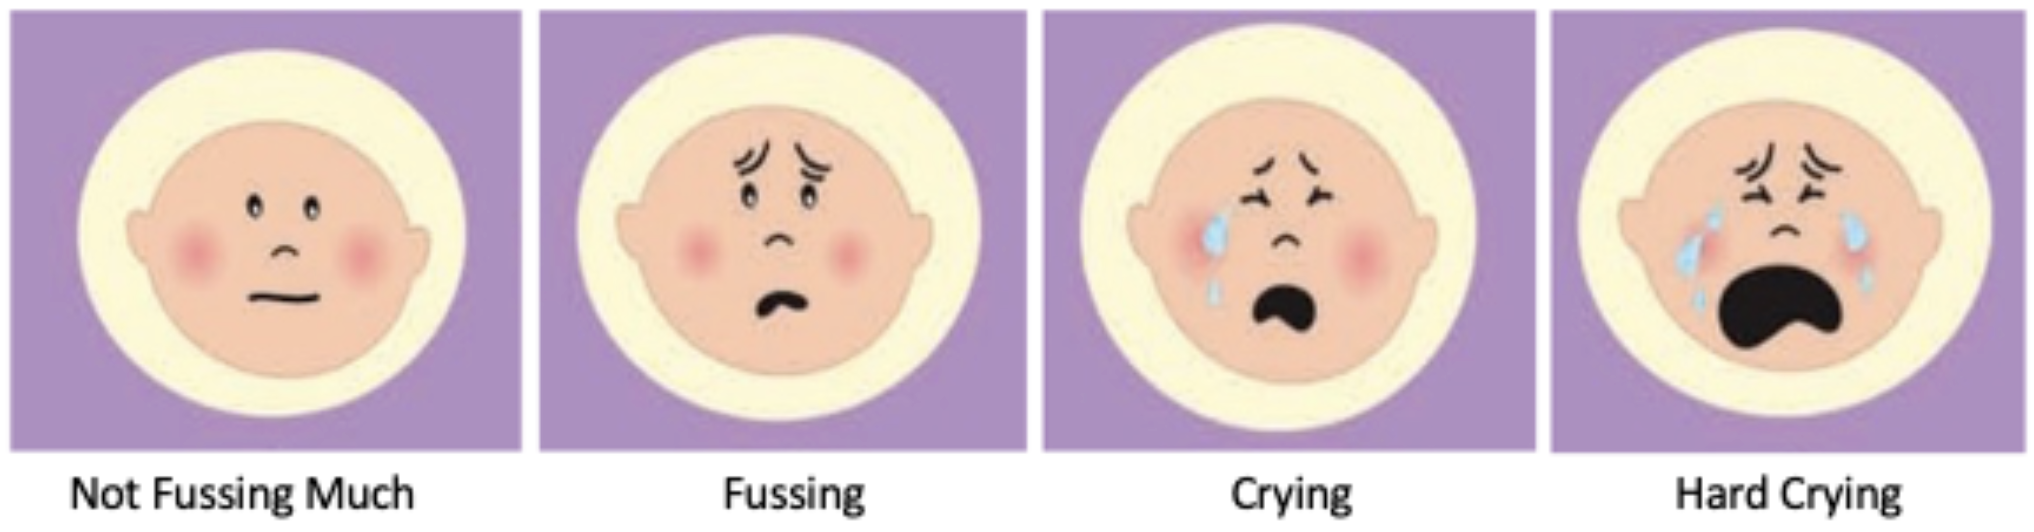
\includegraphics[width=0.5\textwidth,height=\textheight]{../viz/adams_scale.png}

\textbf{9.2.}{[}\emph{If baby was fussy}{]} \textbf{What did you do to
calm BABY down? {[}check all that apply{]}}

\begin{enumerate}
\def\labelenumi{\alph{enumi}.}
\tightlist
\item
  Feed
\item
  Rub or pat
\item
  Swaddle
\item
  Pick up/Bounce/rock/swing
\item
  Shush/white noise
\item
  Play TV/tablet/video/etc
\item
  Play recorded music
\item
  Sing
\item
  Give pacifier / teether
\item
  Put in bed
\item
  Change diaper
\item
  Waited for them to calm down
\item
  Other
\end{enumerate}

\textbf{9.3.} {[}\emph{If baby was fussy}{]} \textbf{How long did it
take BABY to calm down?}

\begin{enumerate}
\def\labelenumi{\alph{enumi}.}
\tightlist
\item
  Less than 1 minute
\item
  1-2 minutes
\item
  3-5 minutes
\item
  6-10 minutes
\item
  11-20 minutes
\item
  20+ minutes (or still fussing)
\end{enumerate}

\textbf{10. Did you sing to BABY in the last 2-3 hours?}

\begin{enumerate}
\def\labelenumi{\alph{enumi}.}
\tightlist
\item
  Yes
\item
  No
\end{enumerate}

\textbf{11. Have you played recorded music for BABY in the last 2-3
hours?}

\begin{enumerate}
\def\labelenumi{\alph{enumi}.}
\tightlist
\item
  Yes
\item
  No
\end{enumerate}

\textbf{12. Have you made or listened to music for your own enjoyment in
the last 2-3 hours?}

\begin{enumerate}
\def\labelenumi{\alph{enumi}.}
\tightlist
\item
  Yes
\item
  No
\end{enumerate}

\subsection*{Supplementary Text 4: Results from Caregiver Exit
Survey}\label{supplementary-text-4-results-from-caregiver-exit-survey}
\addcontentsline{toc}{subsection}{Supplementary Text 4: Results from
Caregiver Exit Survey}

At the end of the study, caregivers were invited to complete an optional
exit survey to share their overall experiences during the 10-week study
period. Fifty-eight caregivers (52.7\%) chose to do so. Summary
information from the survey is presented here.

\subsubsection*{Positive Experiences in the
Study}\label{positive-experiences-in-the-study}
\addcontentsline{toc}{subsubsection}{Positive Experiences in the Study}

The majority of respondents (89.7\%) described their experience
positively, typically mentioning opportunities to actively integrate
music into their daily lives, which they felt led to positive
experiences:

\begin{quote}
\textit{We had a lot of fun singing songs… there was one particular road trip that was challenging [and] I was inspired by the study to sing a lot on to help get us through.}
  
\textit{… She would smile when we sang if she would start to get fussy or be ready for bed. I think it cued her body that she was going to sleep or help soothe her. Really loved the experience! I also felt like the singing bonded us even more!}
  
\textit{I could definitely see that singing to my baby helped soothe him. I really enjoyed the experiment and will keep singing to my baby everyday.}
  
\textit{This study really brought more singing and song-play into my relationship with my son.}
  
\textit{[Baby] responded so well to the signing and would get really excited especially when you're really animated and do actions. It was also helpful when she was unsettled and would calm her quickly.}
  
\textit{[Baby] just loves songs and [it’s] part of our daily routine – I’m not sure if we would have sung as much if we didn’t do the study. She laughs and giggles and particularly loves songs with actions.}
  
\textit{For my own mental health, singing calmed me down and refreshed me almost whilst with my baby it definitely put a smile on her face.}
\end{quote}

\subsubsection*{Views on the Music Enrichment Intervention
Varied}\label{views-on-the-music-enrichment-intervention-varied}
\addcontentsline{toc}{subsubsection}{Views on the Music Enrichment
Intervention Varied}

Consistent with EMA results, most respondents (94.8\%) reported that
they were able to increase singing during the intervention period.
However, while many found the intervention materials helpful for
incorporating more singing into their daily routines, their reactions to
the types of material varied.

For example, fewer than half of the respondents (43.1\%) regularly used
the original songs we produced to broaden caregivers' repertoire for
singing to their infants. Some comments hinted at caregivers' preference
for singing familiar songs rather than learning new songs (e.g., ``I
would have preferred more common children's songs\ldots even if they
were in other languages''; ``I had plenty of my own songs''; ``Just not
my favorite, not very familiar'').

On the other hand, a large number of respondents liked (77.6\%) and
actively used the infant-friendly board book that was sent to
participants, which contained widely popular songs for infants (e.g.,
The Wheels on the Bus, Head Shoulders Knees \& Toes, Twinkle Twinkle
Little Star). The easy accessibility of this physical book (i.e., there
was no need to open and navigate their phone to access songs) also
seemed not only to add convenience for caregivers but also to attract
older siblings of their infants:

\begin{quote}
\textit{My 2yo loved getting involved with singing the songs in the board book!}
  
\textit{My older children enjoyed the board book and began to sing the songs to their sibling too.}
  
\textit{My older child loves the book and frequently uses it to sing with the baby.}
\end{quote}

\subsubsection*{Caregivers' Ability to Complete EMA Surveys
Varied}\label{caregivers-ability-to-complete-ema-surveys-varied}
\addcontentsline{toc}{subsubsection}{Caregivers' Ability to Complete EMA
Surveys Varied}

Some participants found it challenging to respond promptly upon
receiving an EMA ping (34.5\%). When asked to suggest the ideal time for
EMA surveys, 19 respondents recommended when their infants are asleep
(e.g., naptime, nighttime), although, of course, this would be
scientifically counterproductive, in that responses would be
retrospective.

Some parents also noted that due to the complexity of daily life with
young infants, caregivers sometimes had to delay completing surveys
until they had spare moments to complete, even if they noticed the EMA
ping at the moment. There were also instances when caregivers found the
EMA ping had expired at the time when they found a moment to fill out
the survey:

\begin{quote}
\textit{Generally, I responded within 2-4 hrs, as I couldn't guarantee 2 minutes un-interrupted until then.}
  
\textit{Unfortunately the time lapsed on some and was just too busy and would forget to go back to it.}
  
\textit{Difficult juggling baby so sometimes forgot to return once started.}
  
\textit{I didn’t notice the notifications until it was too late and the survey had expired. I wish there was a bigger time window or to notify more prominently.}
  
\textit{It would be good to have more than 4 hours before the survey expired as I wasn't always to complete the survey in that timeframe.}
  
\end{quote}

These responses highlight the challenges caregivers face in promptly
responding to EMA pings while caring for their infants, suggesting the
need for careful consideration in determining EMA schedules.
Nonetheless, the high compliance rate found in the current study,
despite the study asking caregivers to respond to nearly 100 surveys in
10 weeks, suggests that EMA may be a promising method to adopt in
studies of other naturalistic behaviors, especially those amenable to
longitudinal study.

\begin{figure}[p]

{\centering 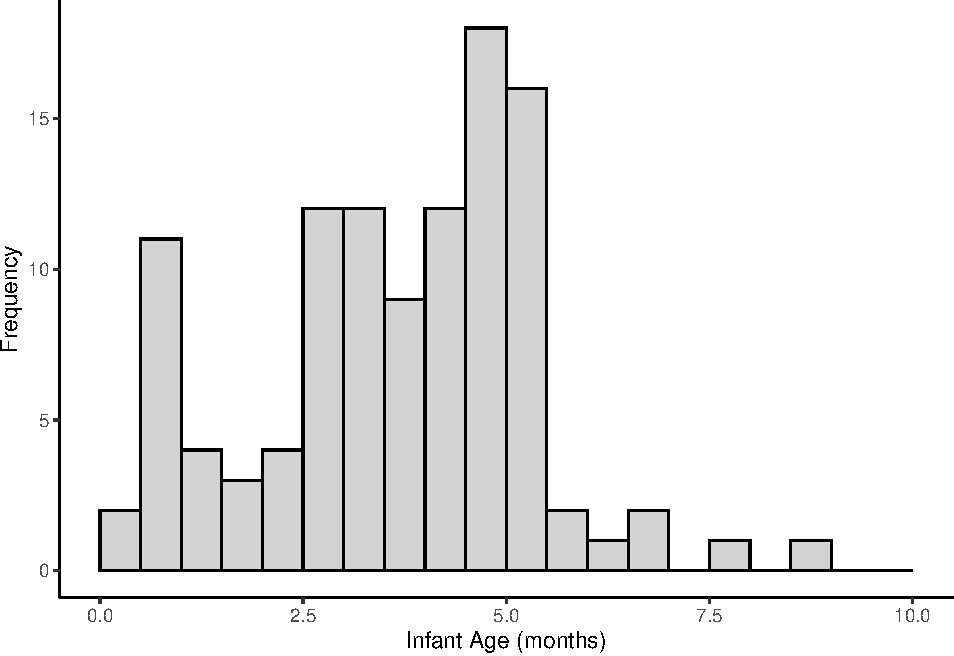
\includegraphics[width=1\linewidth,]{MIPH_childdev_files/figure-latex/supp figure 1-1} 

}

\caption{\textbf{Supplementary Figure 1 | Histogram of infant ages at the start of the study.}}\label{fig:supp figure 1}
\end{figure}

\begin{figure}[p]

{\centering 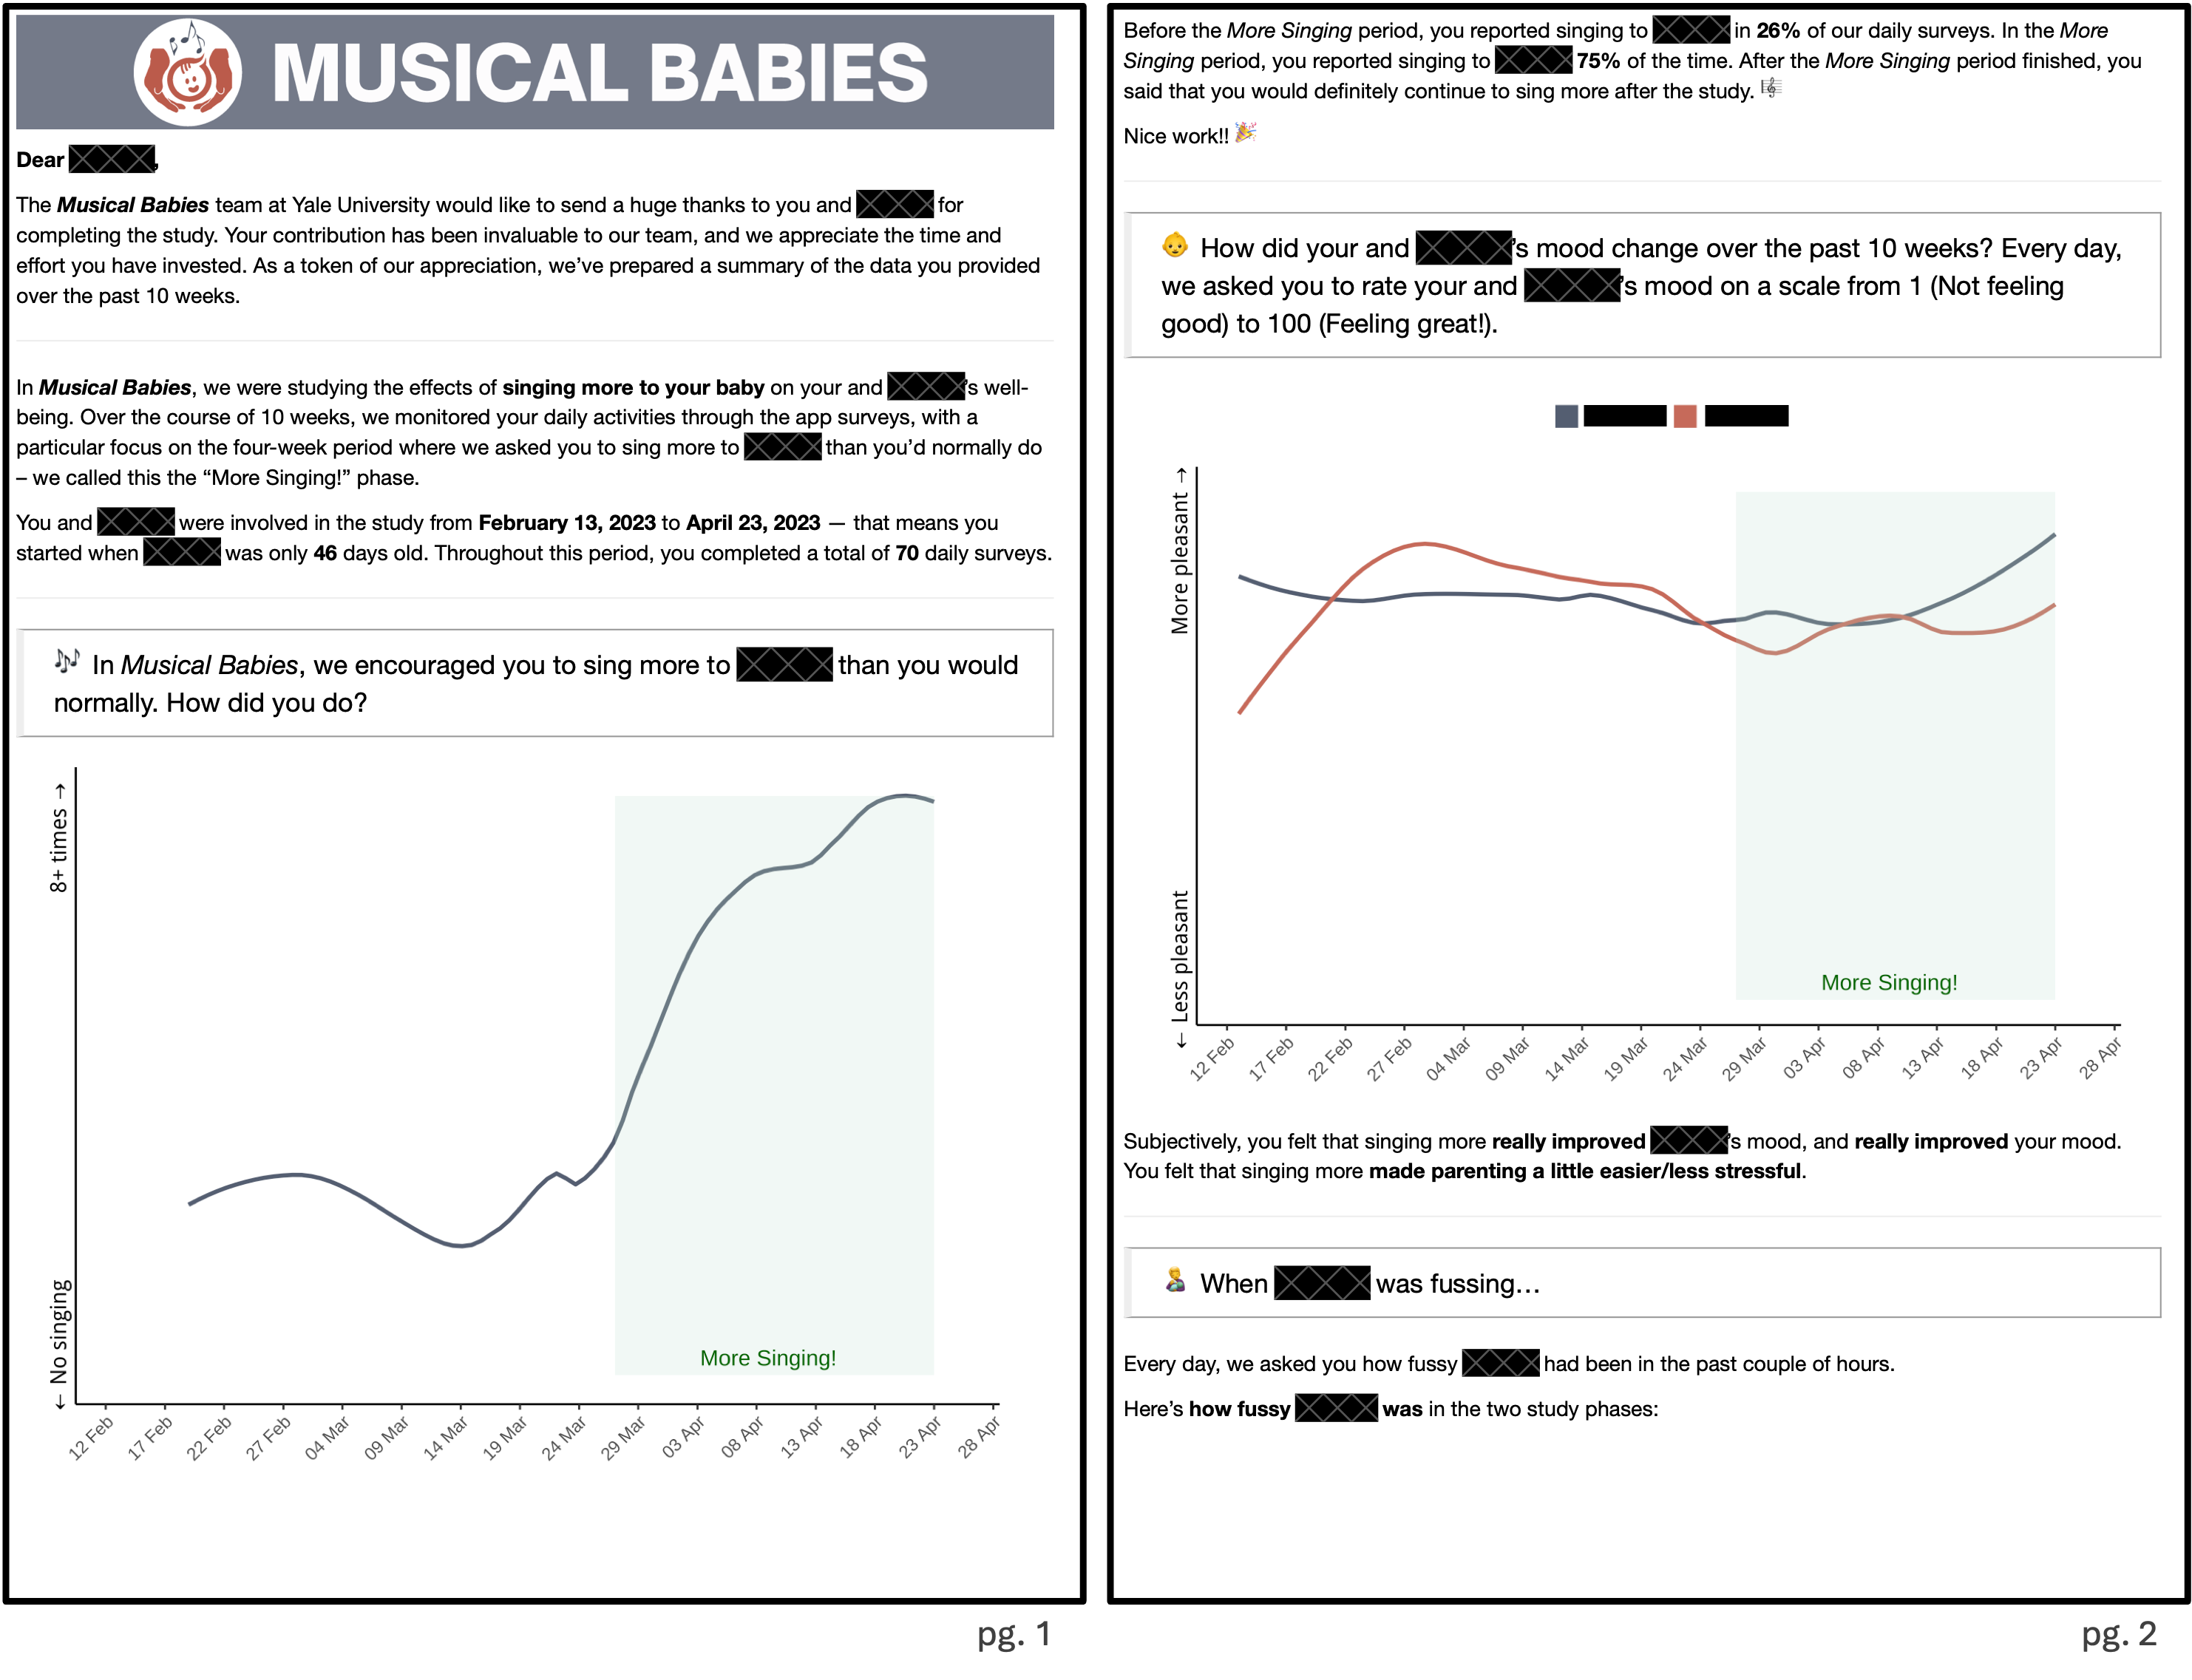
\includegraphics[width=0.9\linewidth,]{../viz/s_figure2a} 

}

\caption{\textbf{Supplementary Figure 2 | Example report for participants.} At the end of the study, we sent participants a report summarizing data they provided over the course of the study, as an incentive.}\label{fig:supp fig 2}
\end{figure}
\begin{figure}[p]

{\centering 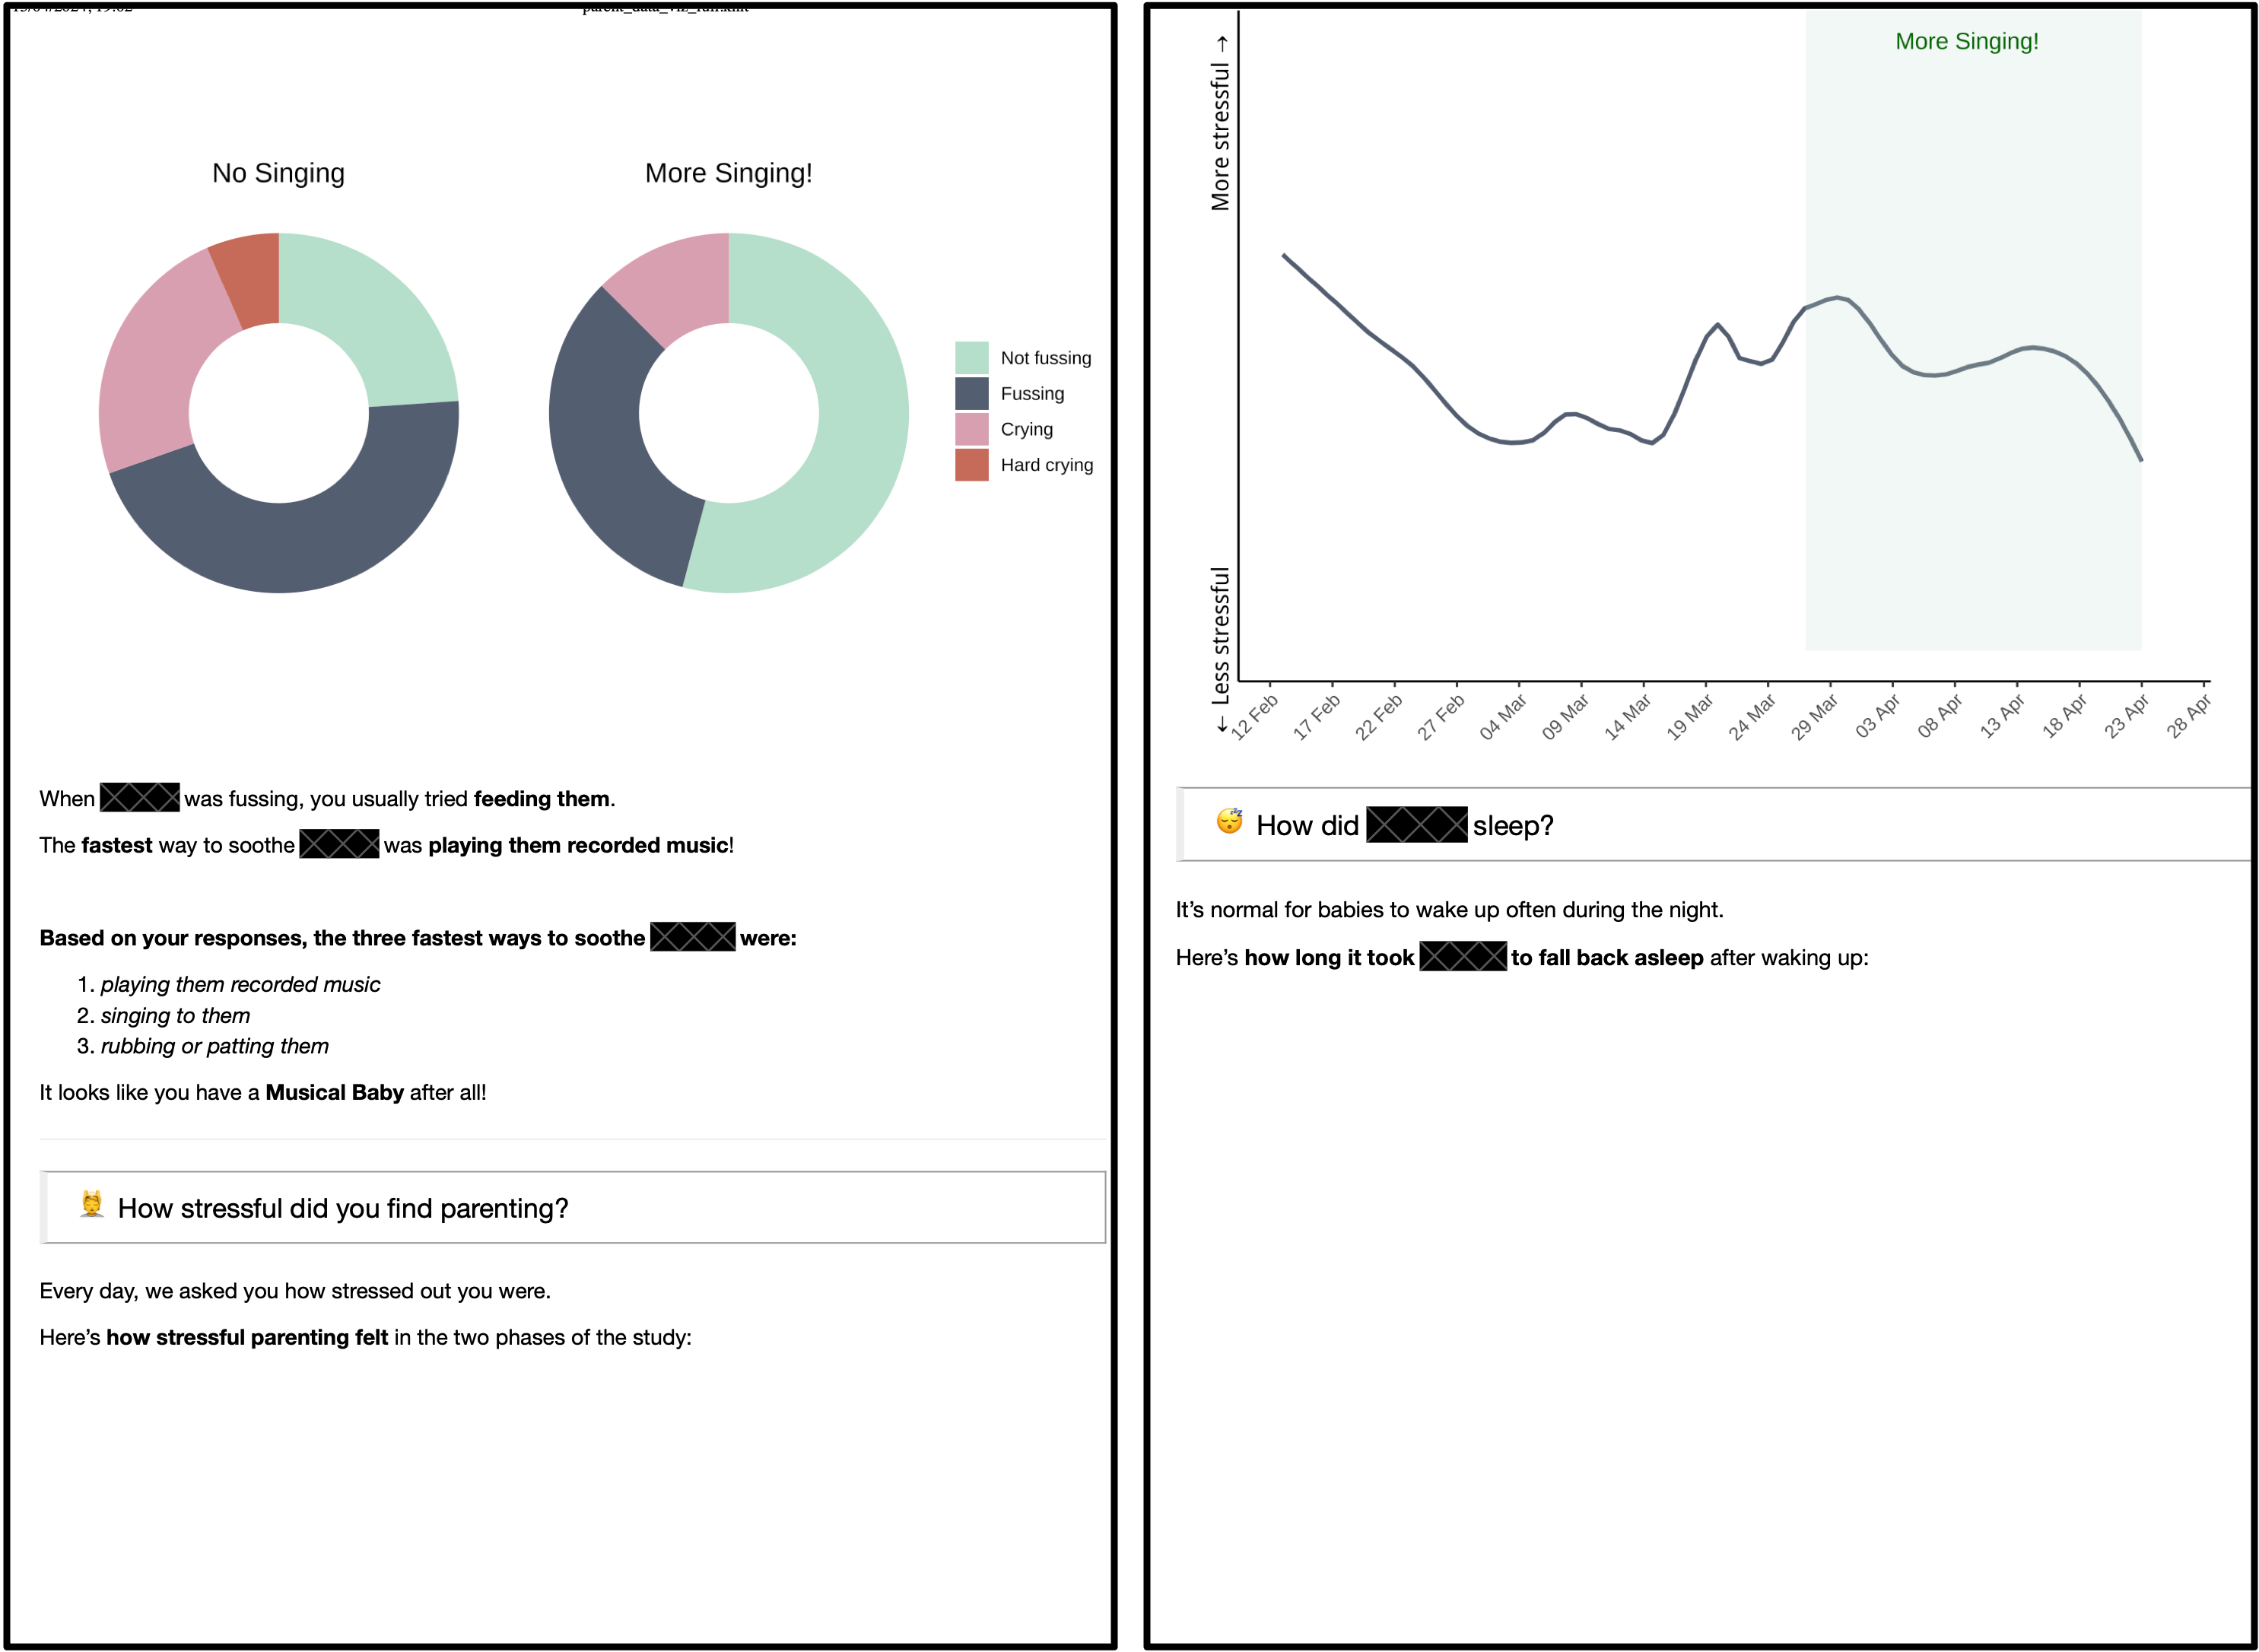
\includegraphics[width=0.9\linewidth,]{../viz/s_figure2b} 

}

\caption{\textbf{Supplementary Figure 2 (cont.) | Example report for participants.}}\label{fig:supp fig 2b}
\end{figure}

\begin{figure}[p]

{\centering 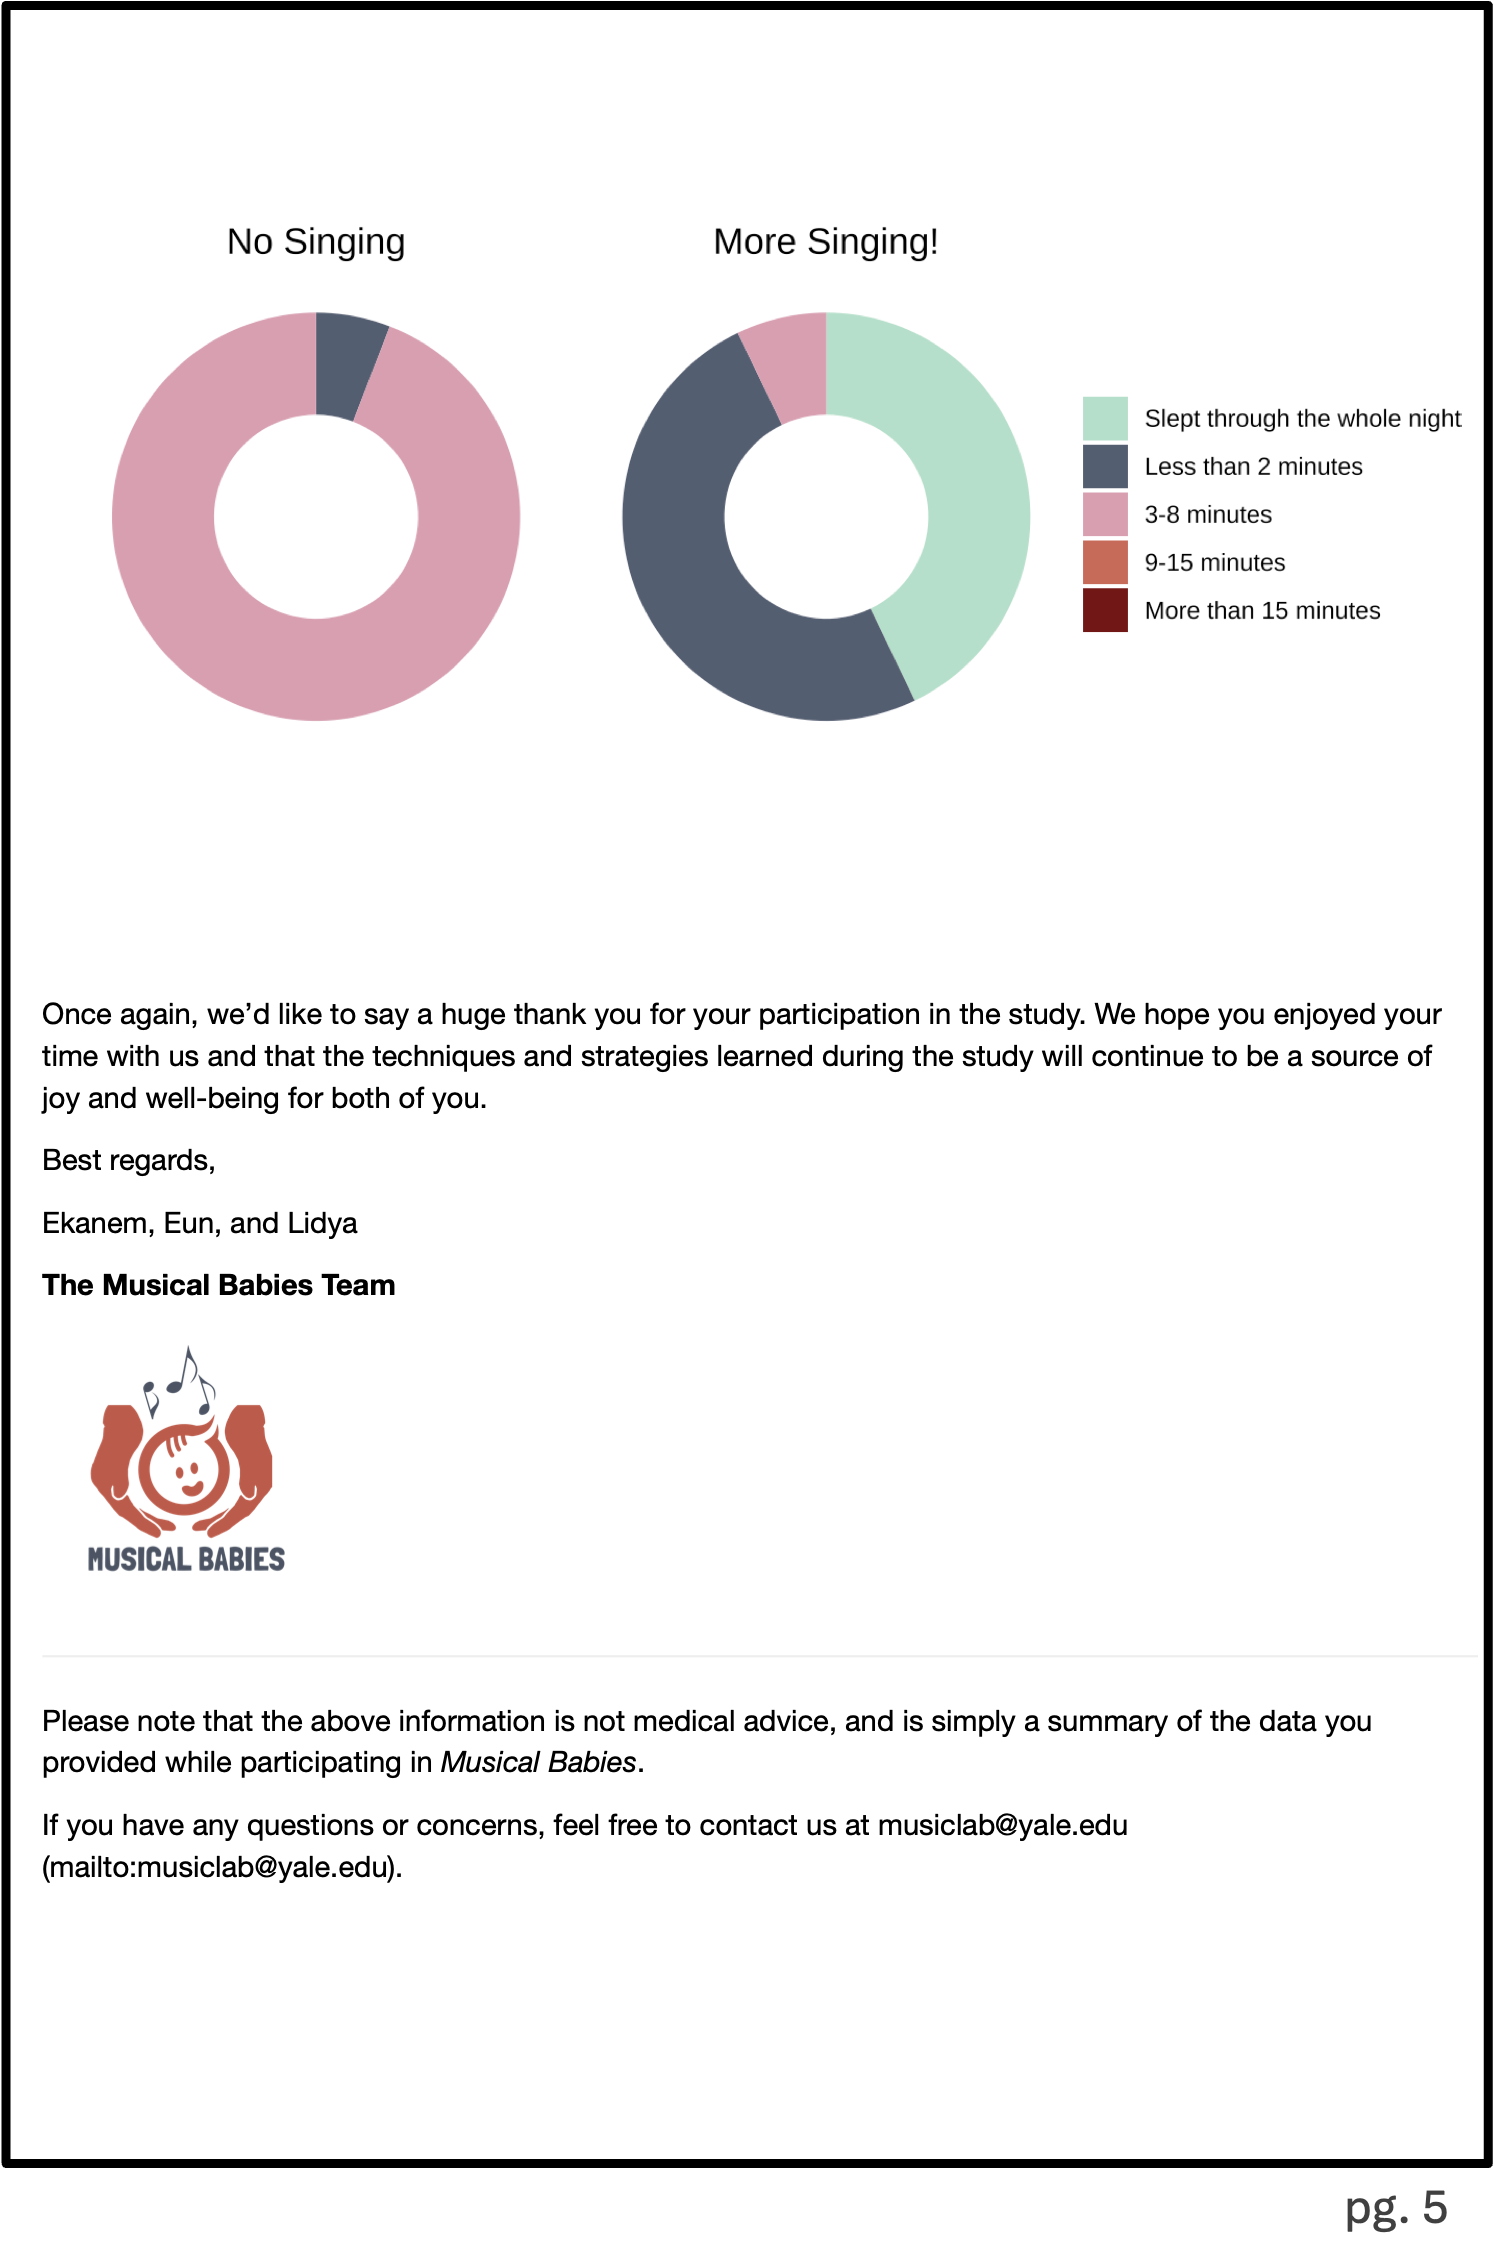
\includegraphics[width=0.5\linewidth,]{../viz/s_figure2c} 

}

\caption{\textbf{Supplementary Figure 2 (cont.) | Example report for participants.}}\label{fig:supp fig 2c}
\end{figure}

\clearpage

\begin{ThreePartTable}
\begin{TableNotes}[para]
\item \textbf{Supplementary Table 1 | Participants' musical backgrounds.} 
\item We measured participants' level of musical training with the question ``How would you describe your music training experience?''. Participants could select any of the following types of musical training: no formal musical training, lessons or classes (either before or during elementary school years, during middle and high school years, or in adulthood), participation in community-based music groups (e.g.,  church choir, community ensembles), majoring in music, and a free-text option. Participants who reported either majoring or minoring in music, or working in music professionally were coded as having an ``advanced''  background in music. We then counted the number of other responses (excluding ``no formal musical training'') selected by each participant, and coded participants as having either ``some''  (< 2 categories selected) or ``intermediate''  (< 4 categories selected) training in music.
\end{TableNotes}
\begin{longtable}{lrr}
\toprule
Level of music training & n & \% of sample\\
\midrule
Advanced & 14 & 12.7\\
\cmidrule{1-3}\pagebreak[0]
Intermediate & 15 & 13.6\\
\cmidrule{1-3}\pagebreak[0]
Some & 63 & 57.3\\
\cmidrule{1-3}\pagebreak[0]
None & 18 & 16.4\\
\bottomrule
\insertTableNotes
\end{longtable}
\end{ThreePartTable}

\clearpage

\begin{ThreePartTable}
\begin{TableNotes}[para]
\item \textbf{Supplementary Table 2 | Demographic characteristics of excluded participants. } 
\item Ten participants were excluded from analyses, either due to dropping out of the study or for low completion rates. Of these participants, we had demographic data from nine.
\end{TableNotes}
\begin{longtable}{llrr}
\toprule
Characteristic &   & n & \% of excluded sample\\
\midrule
 & United States of America & 6 & 66.7\\
\cmidrule{2-4}\nopagebreak
 & New Zealand & 2 & 22.2\\
\cmidrule{2-4}\nopagebreak
\multirow{-3}{*}[1\dimexpr\aboverulesep+\belowrulesep+\cmidrulewidth]{\raggedright\arraybackslash Country of residence} & Canada & 1 & 11.1\\
\cmidrule{1-4}\pagebreak[0]
 & United States of America & 6 & 66.7\\
\cmidrule{2-4}\nopagebreak
 & New Zealand & 2 & 22.2\\
\cmidrule{2-4}\nopagebreak
\multirow{-3}{*}[1\dimexpr\aboverulesep+\belowrulesep+\cmidrulewidth]{\raggedright\arraybackslash Parent's country of birth} & Canada & 1 & 11.1\\
\cmidrule{1-4}\pagebreak[0]
 & White/European/New Zealand European & 7 & 77.8\\
\cmidrule{2-4}\nopagebreak
 & Black or African American & 1 & 11.1\\
\cmidrule{2-4}\nopagebreak
\multirow{-3}{*}[1\dimexpr\aboverulesep+\belowrulesep+\cmidrulewidth]{\raggedright\arraybackslash Parent race/ethnicity} & NA & 1 & 11.1\\
\cmidrule{1-4}\pagebreak[0]
 & College/university graduate & 5 & 55.6\\
\cmidrule{2-4}\nopagebreak
 & Master's degree (MA or equivalent) & 3 & 33.3\\
\cmidrule{2-4}\nopagebreak
\multirow{-3}{*}[1\dimexpr\aboverulesep+\belowrulesep+\cmidrulewidth]{\raggedright\arraybackslash Parent's highest level of education} & Doctoral degree (PhD or equivalent) & 1 & 11.1\\
\cmidrule{1-4}\pagebreak[0]
 & Over \$150,000 & 3 & 33.3\\
\cmidrule{2-4}\nopagebreak
 & \$100,000 to \$150,000 & 3 & 33.3\\
\cmidrule{2-4}\nopagebreak
 & \$50,000 to \$74,999 & 2 & 22.2\\
\cmidrule{2-4}\nopagebreak
\multirow{-4}{*}[1.5\dimexpr\aboverulesep+\belowrulesep+\cmidrulewidth]{\raggedright\arraybackslash Current household income (USD)} & I'd prefer not to say & 1 & 11.1\\
\cmidrule{1-4}\pagebreak[0]
 & 1 & 3 & 33.3\\
\cmidrule{2-4}\nopagebreak
 & 2 & 5 & 55.6\\
\cmidrule{2-4}\nopagebreak
\multirow{-3}{*}[1\dimexpr\aboverulesep+\belowrulesep+\cmidrulewidth]{\raggedright\arraybackslash Number of Children} & 3 & 1 & 11.1\\
\bottomrule
\insertTableNotes
\end{longtable}
\end{ThreePartTable}

\clearpage

\section*{References}\label{references}
\addcontentsline{toc}{section}{References}

\phantomsection\label{refs}
\begin{CSLReferences}{1}{0}
\bibitem[\citeproctext]{ref-Adams2019}
Adams, E. L., Marini, M. E., Brick, T. R., Paul, I. M., Birch, L. L., \&
Savage, J. S. (2019). Ecological momentary assessment of using food to
soothe during infancy in the {INSIGHT} trial. \emph{International
Journal of Behavioral Nutrition and Physical Activity}, \emph{16}(1),
79. \url{https://doi.org/10.1186/s12966-019-0837-y}

\bibitem[\citeproctext]{ref-Allen2018}
Allen, A., Tosun, N., Carlson, S., \& Allen, S. (2018). Postpartum
{Changes} in {Mood} and {Smoking-Related Symptomatology}: {An Ecological
Momentary Assessment Investigation}. \emph{Nicotine \& Tobacco
Research}, \emph{20}(6), 681--689.
\url{https://doi.org/10.1093/ntr/ntx118}

\bibitem[\citeproctext]{ref-Bainbridge2021}
Bainbridge, C. M., Bertolo, M., Youngers, J., Atwood, S., Yurdum, L.,
Simson, J., Lopez, K., Xing, F., Martin, A., \& Mehr, S. A. (2021).
Infants relax in response to unfamiliar foreign lullabies. \emph{Nature
Human Behaviour}. \url{https://doi.org/10.1038/s41562-020-00963-z}

\bibitem[\citeproctext]{ref-Barr1990}
Barr, R. G. (1990). The {Normal Crying Curve}: {What Do We Really Know}?
\emph{Developmental Medicine \& Child Neurology}, \emph{32}(4),
356--362. \url{https://doi.org/10.1111/j.1469-8749.1990.tb16949.x}

\bibitem[\citeproctext]{ref-Bind2023}
Bind, R. H., Sawyer, K., Hazelgrove, K., Rebecchini, L., Miller, C.,
Ahmed, S., Dazzan, P., Sevdalis, N., Bakolis, I., Davis, R., Lopez, M.
B., Woods, A., Crane, N., Manoharan, M., Burton, A., Dye, H., Osborn,
T., Greenwood, L., Perkins, R., \ldots{} Estevao, C. (2023).
Feasibility, clinical efficacy, and well-being outcomes of an online
singing intervention for postnatal depression in the {UK}:
{SHAPER-PNDO}, a single-arm clinical trial. \emph{Pilot and Feasibility
Studies}, \emph{9}(1), 131.
\url{https://doi.org/10.1186/s40814-023-01360-9}

\bibitem[\citeproctext]{ref-Bowlby1969}
Bowlby, J. (1969). \emph{Attachment and loss ({Vol}. {I}:
{Attachment})}. Basic Books.

\bibitem[\citeproctext]{ref-Bradley2002}
Bradley, R. H., \& Corwyn, R. F. (2002). Socioeconomic {Status} and
{Child Development}. \emph{Annual Review of Psychology}, \emph{53}(1),
371--399. \url{https://doi.org/10.1146/annurev.psych.53.100901.135233}

\bibitem[\citeproctext]{ref-Byrn2010}
Byrn, M. D., \& Hourigan, R. (2010). A {Comparative Case Study} of
{Music Interactions Between Mothers} and {Infants}. \emph{Contributions
to Music Education}, \emph{37}(1), 65--79.

\bibitem[\citeproctext]{ref-Cho2021}
Cho, E., \& Ilari, B. S. (2021). Mothers as home {DJs}: {Recorded} music
and young children's well-being during the {Covid-19} pandemic.
\emph{Frontiers in Psychology}, \emph{12}, 637569.
\url{https://doi.org/10.3389/fpsyg.2021.637569}

\bibitem[\citeproctext]{ref-Cirelli2020a}
Cirelli, L. K., Jurewicz, Z. B., \& Trehub, S. E. (2020). Effects of
{Maternal Singing Style} on {Mother}--{Infant Arousal} and {Behavior}.
\emph{Journal of Cognitive Neuroscience}, \emph{32}(7), 1213--1220.
\url{https://doi.org/10.1162/jocn_a_01402}

\bibitem[\citeproctext]{ref-Cirelli2020}
Cirelli, L. K., \& Trehub, S. E. (2020). Familiar songs reduce infant
distress. \emph{Developmental Psychology}.
\url{https://doi.org/10.1037/dev0000917}

\bibitem[\citeproctext]{ref-Corbeil2016}
Corbeil, M., Trehub, S. E., \& Peretz, I. (2016). Singing delays the
onset of infant distress. \emph{Infancy : The Official Journal of the
International Society on Infant Studies}, \emph{21}(3), 373--391.
\url{https://doi.org/10.1111/infa.12114}

\bibitem[\citeproctext]{ref-Corpuz2023}
Corpuz, R., Kotov, D. A., \& Donovan, R. L. (2023). Earlier sexual debut
predicts higher (not lower) levels of father care measured across 12
weeks: {An} experience sampling study. \emph{Frontiers in Psychology},
\emph{14}, 1199735. \url{https://doi.org/10.3389/fpsyg.2023.1199735}

\bibitem[\citeproctext]{ref-Cox1987}
Cox, J. L., Holden, J. M., \& Sagovsky, R. (1987). Detection of
postnatal depression: {Development} of the 10-item {Edinburgh Postnatal
Depression Scale}. \emph{British Journal of Psychiatry}, \emph{150}(6),
782--786. \url{https://doi.org/10.1192/bjp.150.6.782}

\bibitem[\citeproctext]{ref-Custodero2003}
Custodero, L. A., \& Johnson-Green, E. A. (2003). Passing the cultural
torch: {Musical} experience and musical parenting of infants.
\emph{Journal of Research in Music Education}, \emph{51}(2), 102--114.
\url{https://doi.org/10.2307/3345844}

\bibitem[\citeproctext]{ref-Custodero2003a}
Custodero, L. A., Rebello Britto, P., \& Brooks-Gunn, J. (2003). Musical
lives: {A} collective portrait of {American} parents and their young
children. \emph{Journal of Applied Developmental Psychology},
\emph{24}(5), 553--572.
\url{https://doi.org/10.1016/j.appdev.2003.08.005}

\bibitem[\citeproctext]{ref-deBarbaro2023}
de Barbaro, K., Micheletti, M., Yao, X., Khante, P., Johnson, M., \&
Goodman, S. (2023). Infant crying predicts real-time fluctuations in
maternal mental health in ecologically valid home settings.
\emph{Developmental Psychology}, \emph{59}(4), 733--744.
\url{https://doi.org/10.1037/dev0001530}

\bibitem[\citeproctext]{ref-Dennis2006}
Dennis, C.-L., \& Ross, L. (2006). Women's perceptions of partner
support and conflict in the development of postpartum depressive
symptoms. \emph{Journal of Advanced Nursing}, \emph{56}(6), 588--599.
\url{https://doi.org/10.1111/j.1365-2648.2006.04059.x}

\bibitem[\citeproctext]{ref-Dora2024}
Dora, J., Kuczynski, A. M., Schultz, M. E., Acuff, S. F., Murphy, J. G.,
\& King, K. M. (2024). An experimental investigation into the effect of
negative affect on the behavioral economic demand for alcohol.
\emph{Psychology of Addictive Behaviors}.

\bibitem[\citeproctext]{ref-Fancourt2018a}
Fancourt, D., \& Perkins, R. (2018a). Effect of singing interventions on
symptoms of postnatal depression: {Three-arm} randomised controlled
trial. \emph{The British Journal of Psychiatry}, 1--3.
\url{https://doi.org/10.1192/bjp.2017.29}

\bibitem[\citeproctext]{ref-Fancourt2018c}
Fancourt, D., \& Perkins, R. (2018b). The effects of mother--infant
singing on emotional closeness, affect, anxiety, and stress hormones.
\emph{Music \& Science}, \emph{1}, 205920431774574.
\url{https://doi.org/10.1177/2059204317745746}

\bibitem[\citeproctext]{ref-Fancourt2018}
Fancourt, D., \& Perkins, R. (2018c). Maternal engagement with music up
to nine months post-birth: {Findings} from a cross-sectional study in
{England}. \emph{Psychology of Music}, \emph{46}(2), 238--251.
\url{https://doi.org/10.1177/0305735617705720}

\bibitem[\citeproctext]{ref-Feldman2009}
Feldman, R., Granat, A., Pariente, C., Kanety, H., Kuint, J., \&
Gilboa-Schechtman, E. (2009). Maternal depression and anxiety across the
postpartum year and infant social engagement, fear regulation, and
stress reactivity. \emph{Journal of the American Academy of Child \&
Adolescent Psychiatry}, \emph{48}(9), 919--927.
\url{https://doi.org/10.1097/CHI.0b013e3181b21651}

\bibitem[\citeproctext]{ref-Feldman2014}
Feldman, R., Rosenthal, Z., \& Eidelman, A. I. (2014). Maternal-preterm
skin-to-skin contact enhances child physiologic organization and
cognitive control across the first 10 years of life. \emph{Biological
Psychiatry}, \emph{75}(1), 56--64.
\url{https://doi.org/10.1016/j.biopsych.2013.08.012}

\bibitem[\citeproctext]{ref-Franchak2019}
Franchak, J. M. (2019). Changing {Opportunities} for {Learning} in
{Everyday Life}: {Infant Body Position Over} the {First Year}.
\emph{Infancy : The Official Journal of the International Society on
Infant Studies}, \emph{24}(2), 187--209.
\url{https://doi.org/10.1111/infa.12272}

\bibitem[\citeproctext]{ref-Franchak2024}
Franchak, J. M., Kadooka, K., \& Fausey, C. M. (2024). Longitudinal
relations between independent walking, body position, and object
experiences in home life. \emph{Developmental Psychology}, \emph{60}(2),
228--242. \url{https://doi.org/10.1037/dev0001678}

\bibitem[\citeproctext]{ref-Fries2005}
Fries, A. B. W., Ziegler, T. E., Kurian, J. R., Jacoris, S., \& Pollak,
S. D. (2005). Early experience in humans is associated with changes in
neuropeptides critical for regulating social behavior. \emph{Proceedings
of the National Academy of Sciences}, \emph{102}(47), 17237--17240.
\url{https://doi.org/10.1073/pnas.0504767102}

\bibitem[\citeproctext]{ref-Gerry2012}
Gerry, D., Unrau, A., \& Trainor, L. J. (2012). Active music classes in
infancy enhance musical, communicative and social development.
\emph{Developmental Science}, \emph{15}(3), 398--407.
\url{https://doi.org/10.1111/j.1467-7687.2012.01142.x}

\bibitem[\citeproctext]{ref-Hilton2022a}
Hilton, C. B., Moser, C. J., Bertolo, M., Lee-Rubin, H., Amir, D.,
Bainbridge, C. M., Simson, J., Knox, D., Glowacki, L., Alemu, E.,
Galbarczyk, A., Jasienska, G., Ross, C. T., Neff, M. B., Martin, A.,
Cirelli, L. K., Trehub, S. E., Song, J., Kim, M., \ldots{} Mehr, S. A.
(2022). Acoustic regularities in infant-directed speech and song across
cultures. \emph{Nature Human Behaviour}.
\url{https://doi.org/10.1101/2020.04.09.032995}

\bibitem[\citeproctext]{ref-Hippe2024}
Hippe, L., Hennessy, V., Ramirez, N. F., \& Zhao, T. C. (2024).
Comparison of speech and music input in {North American} infants' home
environment over the first 2 years of life. \emph{Developmental
Science}, \emph{27}(5), e13528. \url{https://doi.org/10.1111/desc.13528}

\bibitem[\citeproctext]{ref-Ilari2005}
Ilari, B. (2005). On musical parenting of young children: {Musical}
beliefs and behaviors of mothers and infants. \emph{Early Child
Development and Care}, \emph{175}(7-8), 647--660.
\url{https://doi.org/10.1080/0300443042000302573}

\bibitem[\citeproctext]{ref-Kotler2019}
Kotler, J., Mehr, S. A., Egner, A., Haig, D., \& Krasnow, M. M. (2019).
Response to vocal music in {Angelman} syndrome contrasts with
{Prader-Willi} syndrome. \emph{Evolution and Human Behavior},
\emph{40}(5), 420--426.
\url{https://doi.org/10.1016/j.evolhumbehav.2019.05.003}

\bibitem[\citeproctext]{ref-Kuczynski2024}
Kuczynski, A. M., Piccirillo, M. L., Dora, J., Kuehn, K. S., Halvorson,
M. A., King, K. M., \& Kanter, J. W. (2024). Characterizing the
momentary association between loneliness, depression, and social
interactions: {Insights} from an ecological momentary assessment study.
\emph{Journal of Affective Disorders}, \emph{360}, 376--386.
\url{https://doi.org/10.1016/j.jad.2024.05.148}

\bibitem[\citeproctext]{ref-Lense2022}
Lense, M. D., Shultz, S., Astésano, C., \& Jones, W. (2022). Music of
infant-directed singing entrains infants' social visual behavior.
\emph{Proceedings of the National Academy of Sciences}, \emph{119}(45),
e2116967119. \url{https://doi.org/10.1073/pnas.2116967119}

\bibitem[\citeproctext]{ref-Lerma-Arregoces2024}
Lerma-Arregocés, D., \& Pérez-Moreno, J. (2024). Musical communication
among parents and their children: {An} analysis tool to study their
interaction. \emph{International Journal of Music Education},
\emph{42}(3), 409--424. \url{https://doi.org/10.1177/02557614231174033}

\bibitem[\citeproctext]{ref-Liu2023}
Liu, J., Hilton, C. B., Bergelson, E., \& Mehr, S. A. (2023). Language
experience predicts music processing in a half-million speakers of
fifty-four languages. \emph{Current Biology}, \emph{33}(10),
1916--1925.e4. \url{https://doi.org/10.1016/j.cub.2023.03.067}

\bibitem[\citeproctext]{ref-Long2023}
Long, B., Simson, J., Buxó-Lugo, A., Watson, D. G., \& Mehr, S. A.
(2023). How games can make behavioural science better. \emph{Nature},
\emph{613}(7944), 433--436.
\url{https://doi.org/10.1038/d41586-023-00065-6}

\bibitem[\citeproctext]{ref-Malloch1999}
Malloch, S. N. (1999). Mothers and infants and communicative musicality.
\emph{Musicae Scientiae}, \emph{3}(1\_suppl), 29--57.
\url{https://doi.org/10.1177/10298649000030S104}

\bibitem[\citeproctext]{ref-Malloch2009}
Malloch, S. N., \& Trevarthen, C. (2009). \emph{Communicative
musicality: {Exploring} the basis of human companionship}. Oxford
University Press.

\bibitem[\citeproctext]{ref-Mehr2014}
Mehr, S. A. (2014). Music in the home: {New} evidence for an
intergenerational link. \emph{Journal of Research in Music Education},
\emph{62}(1), 78--88. \url{https://doi.org/10.1177/0022429413520008}

\bibitem[\citeproctext]{ref-Mehr2017b}
Mehr, S. A., Kotler, J., Howard, R. M., Haig, D., \& Krasnow, M. M.
(2017). Genomic imprinting is implicated in the psychology of music.
\emph{Psychological Science}, \emph{28}(10), 1455--1467.
\url{https://doi.org/10.1177/0956797617711456}

\bibitem[\citeproctext]{ref-Mehr2017a}
Mehr, S. A., \& Krasnow, M. M. (2017). Parent-offspring conflict and the
evolution of infant-directed song. \emph{Evolution and Human Behavior},
\emph{38}(5), 674--684.
\url{https://doi.org/10.1016/j.evolhumbehav.2016.12.005}

\bibitem[\citeproctext]{ref-Mehr2021}
Mehr, S. A., Krasnow, M. M., Bryant, G. A., \& Hagen, E. H. (2021).
Origins of music in credible signaling. \emph{Behavioral and Brain
Sciences}, \emph{44}, e60.
\url{https://doi.org/10.1017/S0140525X20000345}

\bibitem[\citeproctext]{ref-Mehr2019}
Mehr, S. A., Singh, M., Knox, D., Ketter, D. M., Pickens-Jones, D.,
Atwood, S., Lucas, C., Jacoby, N., Egner, A. A., Hopkins, E. J., Howard,
R. M., Hartshorne, J. K., Jennings, M. V., Simson, J., Bainbridge, C.
M., Pinker, S., O'Donnell, T. J., Krasnow, M. M., \& Glowacki, L.
(2019). Universality and diversity in human song. \emph{Science},
\emph{366}(6468), 957--970.
\url{https://doi.org/10.1126/science.aax0868}

\bibitem[\citeproctext]{ref-Mehr2016}
Mehr, S. A., Song, L. A., \& Spelke, E. S. (2016). For 5-month-old
infants, melodies are social. \emph{Psychological Science},
\emph{27}(4), 486--501. \url{https://doi.org/10.1177/0956797615626691}

\bibitem[\citeproctext]{ref-Mehr2017c}
Mehr, S. A., \& Spelke, E. S. (2017). Shared musical knowledge in
11-month-old infants. \emph{Developmental Science}, \emph{21}(2).
\url{https://doi.org/10.1111/desc.12542}

\bibitem[\citeproctext]{ref-Mendoza2021}
Mendoza, J. K., \& Fausey, C. M. (2021). Everyday music in infancy.
\emph{Developmental Science}.
\url{https://doi.org/10.31234/osf.io/sqatb}

\bibitem[\citeproctext]{ref-Moore2012}
Moore, E. R., Anderson, G. C., Bergman, N., \& Dowswell, T. (2012).
Early skin-to-skin contact for mothers and their healthy newborn
infants. In The Cochrane Collaboration (Ed.), \emph{Cochrane {Database}
of {Systematic Reviews}} (p. CD003519.pub3). John Wiley \& Sons, Ltd.
\url{https://doi.org/10.1002/14651858.CD003519.pub3}

\bibitem[\citeproctext]{ref-Nolvi2016}
Nolvi, S., Karlsson, L., Bridgett, D. J., Pajulo, M., Tolvanen, M., \&
Karlsson, H. (2016). Maternal postnatal psychiatric symptoms and infant
temperament affect early mother-infant bonding. \emph{Infant Behavior
and Development}, \emph{43}, 13--23.
\url{https://doi.org/10.1016/j.infbeh.2016.03.003}

\bibitem[\citeproctext]{ref-Oddi2013}
Oddi, K. B., Murdock, K. W., Vadnais, S., Bridgett, D. J., \& Gartstein,
M. A. (2013). Maternal and {Infant Temperament Characteristics} as
{Contributors} to {Parenting Stress} in the {First Year Postpartum}.
\emph{Infant and Child Development}, \emph{22}(6), 553--579.
\url{https://doi.org/10.1002/icd.1813}

\bibitem[\citeproctext]{ref-Perkel2020}
Perkel, J. M. (2020). Mischief-making bots attacked my scientific
survey. \emph{Nature}, \emph{579}(7799), 461--461.
\url{https://doi.org/10.1038/d41586-020-00768-0}

\bibitem[\citeproctext]{ref-Perkins2018}
Perkins, R., Yorke, S., \& Fancourt, D. (2018). How group singing
facilitates recovery from the symptoms of postnatal depression: A
comparative qualitative study. \emph{BMC Psychology}, \emph{6}(1), 41.
\url{https://doi.org/10.1186/s40359-018-0253-0}

\bibitem[\citeproctext]{ref-Persico2017}
Persico, G., Antolini, L., Vergani, P., Costantini, W., Nardi, M. T., \&
Bellotti, L. (2017). Maternal singing of lullabies during pregnancy and
after birth: {Effects} on mother--infant bonding and on newborns'
behaviour. {Concurrent Cohort Study}. \emph{Women and Birth},
\emph{30}(4), e214--e220.
\url{https://doi.org/10.1016/j.wombi.2017.01.007}

\bibitem[\citeproctext]{ref-Reid2015}
Reid, K. M., \& Taylor, M. G. (2015). Social support, stress, and
maternal postpartum depression: {A} comparison of supportive
relationships. \emph{Social Science Research}, \emph{54}, 246--262.
\url{https://doi.org/10.1016/j.ssresearch.2015.08.009}

\bibitem[\citeproctext]{ref-Reis2012}
Reis, H. T. (2012). Why researchers should think "real-world": {A}
conceptual rationale. In \emph{Handbook of research methods for studying
daily life.} (pp. 3--21). The Guilford Press.

\bibitem[\citeproctext]{ref-Roubinov2017}
Roubinov, D. S., \& Boyce, W. T. (2017). Parenting and {SES}: {Relative}
values or enduring principles? \emph{Current Opinion in Psychology},
\emph{15}, 162--167. \url{https://doi.org/10.1016/j.copsyc.2017.03.001}

\bibitem[\citeproctext]{ref-Schore2005}
Schore, A. N. (2005). Back to basics. \emph{Pediatrics In Review},
\emph{26}(6), 204--217. \url{https://doi.org/10.1542/pir.26.6.204}

\bibitem[\citeproctext]{ref-Shaw2005}
Shaw, S. K., \& Dallos, R. (2005). Attachment and adolescent depression:
{The} impact of early attachment experiences. \emph{Attachment \& Human
Development}, \emph{7}(4), 409--424.
\url{https://doi.org/10.1080/14616730500365902}

\bibitem[\citeproctext]{ref-Shenfield2003}
Shenfield, T., Trehub, S. E., \& Nakata, T. (2003). Maternal singing
modulates infant arousal. \emph{Psychology of Music}, \emph{31}(4),
365--375. \url{https://doi.org/10.1177/0305735603031400}

\bibitem[\citeproctext]{ref-Shonkoff2012}
Shonkoff, J. P., Garner, A. S., Siegel, B. S., Dobbins, M. I., Earls, M.
F., Garner, A. S., McGuinn, L., Pascoe, J., \& Wood, D. L. (2012). The
lifelong effects of early childhood adversity and toxic stress.
\emph{Pediatrics}, \emph{129}(1), e232--e246.
\url{https://doi.org/10.1542/peds.2011-2663}

\bibitem[\citeproctext]{ref-Singh2023}
Singh, M., \& Mehr, S. A. (2023). Universality, domain-specificity and
development of psychological responses to music. \emph{Nature Reviews
Psychology}, 1--14. \url{https://doi.org/10.1038/s44159-023-00182-z}

\bibitem[\citeproctext]{ref-Smith2024}
Smith, A. R., Salley, B., Hanson-Abromeit, D., Paluch, R. A., Engel, H.,
Piazza, J., \& Kong, K. L. (2024). The impact of a community-based music
program during infancy on the quality of parent--child language
interactions. \emph{Child Development}, \emph{95}(2), 481--496.
\url{https://doi.org/10.1111/cdev.14005}

\bibitem[\citeproctext]{ref-Stams2002}
Stams, G.-J. J. M., Juffer, F., \& van IJzendoorn, M. H. (2002).
Maternal sensitivity, infant attachment, and temperament in early
childhood predict adjustment in middle childhood: {The} case of adopted
children and their biologically unrelated parents. \emph{Developmental
Psychology}, \emph{38}(5), 806--821.
\url{https://doi.org/10.1037/0012-1649.38.5.806}

\bibitem[\citeproctext]{ref-Steele2008}
Steele, H., Steele, M., \& Croft, C. (2008). Early attachment predicts
emotion recognition at 6 and 11 years old. \emph{Attachment \& Human
Development}, \emph{10}(4), 379--393.
\url{https://doi.org/10.1080/14616730802461409}

\bibitem[\citeproctext]{ref-Steinberg2021}
Steinberg, S., Shivers, C. M., Liu, T., Cirelli, L. K., \& Lense, M. D.
(2021). Survey of the home music environment of children with various
developmental profiles. \emph{Journal of Applied Developmental
Psychology}, \emph{75}, 101296.
\url{https://doi.org/10.1016/j.appdev.2021.101296}

\bibitem[\citeproctext]{ref-Stone2002}
Stone, A. A., \& Shiffman, S. (2002). Capturing momentary, self-report
data: {A} proposal for reporting guidelines. \emph{Annals of Behavioral
Medicine}, \emph{24}(3), 236--243.
\url{https://doi.org/10.1207/S15324796ABM2403_09}

\bibitem[\citeproctext]{ref-Stone2007}
Stone, A. A., Shiffman, S., Atienza, A. A., Nebeling, L., Stone, A.,
Shiffman, S., Atienza, A. A., \& Nebeling, L. (2007). Historical roots
and rationale of ecological momentary assessment ({EMA}). \emph{The
Science of Real-Time Data Capture: Self-Reports in Health Research},
3--10.

\bibitem[\citeproctext]{ref-Takacs2020}
Takács, L., Smolík, F., Kaźmierczak, M., \& Putnam, S. P. (2020). Early
infant temperament shapes the nature of mother-infant bonding in the
first postpartum year. \emph{Infant Behavior and Development},
\emph{58}, 101428. \url{https://doi.org/10.1016/j.infbeh.2020.101428}

\bibitem[\citeproctext]{ref-Thornton2020}
Thornton, M. A., \& Tamir, D. I. (2020). People represent mental states
in terms of rationality, social impact, and valence: {Validating} the 3d
{Mind Model}. \emph{Cortex; a Journal Devoted to the Study of the
Nervous System and Behavior}, \emph{125}, 44--59.
\url{https://doi.org/10.1016/j.cortex.2019.12.012}

\bibitem[\citeproctext]{ref-Trehub2019}
Trehub, S. E., \& Gudmundsdottir, H. R. (2019). Mothers as singing
mentors for infants. In \emph{The {Oxford} handbook of singing} (pp.
454--470). Oxford University Press.
\url{https://doi.org/10.1093/oxfordhb/9780199660773.013.25}

\bibitem[\citeproctext]{ref-Trehub2006}
Trehub, S. E., \& Hannon, E. E. (2006). Infant music perception:
{Domain-general} or domain-specific mechanisms? \emph{Cognition},
\emph{100}(1), 73--99.
\url{https://doi.org/10.1016/j.cognition.2005.11.006}

\bibitem[\citeproctext]{ref-vandenHeuvel2021}
van den Heuvel, M., Bülow, A., Heininga, V., de Moor, L., Janssen, L.,
Abeele, M., \& Boekhorst, M. (2021). Tracking {Infant Development With}
a {Smartphone}: {A Practical Guide} to the {Experience Sampling Method}.
\emph{Frontiers in Psychology}, \emph{12}.
\url{https://doi.org/10.3389/fpsyg.2021.703743}

\bibitem[\citeproctext]{ref-Wenze2023}
Wenze, S. J., Battle, C. L., Huntley, E. D., Gaugler, T. L., \& Kats, D.
(2023). Ecological momentary assessment of postpartum outcomes in
mothers of multiples: {Lower} maternal-infant bonding, higher stress,
and more disrupted sleep. \emph{Archives of Women's Mental Health},
\emph{26}(3), 361--378. \url{https://doi.org/10.1007/s00737-023-01317-0}

\bibitem[\citeproctext]{ref-Yan2021}
Yan, R., Jessani, G., Spelke, E., de Villiers, P., de Villiers, J., \&
Mehr, S. (2021). Across demographics and recent history, most parents
sing to their infants and toddlers daily. \emph{Philosophical
Transactions of the Royal Society B: Biological Sciences},
\emph{376}(20210089).

\bibitem[\citeproctext]{ref-Yurdum2023}
Yurdum, L., Singh, M., Glowacki, L., Vardy, T., Atkinson, Q. D., Hilton,
C. B., Sauter, D., Krasnow, M. M., \& Mehr, S. A. (2023). Universal
interpretations of vocal music. \emph{Proceedings of the National
Academy of Sciences}, \emph{120}(37), e2218593120.
\url{https://doi.org/10.1073/pnas.2218593120}

\end{CSLReferences}

\end{document}
